\chapter{Implementace platformy}

\section{Konverzní mechanismus}

Prvním krokem ve vývoji konverzního modulu je volba a analýza zdrojové platformy. Je třeba zpracovat danou doménu a především se seznámit se strukturou datového modelu. Druhým krokem je tvorba R2RML mapovacího skriptu. Závěrečným krokem je samotná implementace konverzního mechanismu. Tento postup uvádíme proto, že jednotlivé kroky lze řešit nezávisle. Např. definované R2RML mapování nad konkrétní doménou může posloužit jako podklad k různým aplikacím pracujícím s R2RML. 

\subsection{Munis ESML}

Jako zdroj pro implementaci konverzního mechanismu byl zvolen modul Munis ESML. Jedná se o část informačního systému pro města a obce společnosti Triada. spol. s.r.o.

Účelem modulu Munis ESML je evidování odběratelských i dodavatelských smluv. Nabízí přehledné vyhledávání, statistiky, hlídání termínů, nebo možnost přiřadit smlouvy jednotlivým grantům, projektům či veřejným zakázkám (viz. Obr \ref{obr:munisEsml}).

\begin{figure}[H]
\centerline{\includegraphics[width=\textwidth]{img/munisEsml.eps}}
\caption{Modul ESML}
\label{obr:munisEsml}
\end{figure}

\newpage

\subsubsection{Struktura datového modelu}

Základem datového modelu jsou entity \textit{Smlouva} a \textit{Verze smlouvy}. Smlouva je základním stavovým objektem s hierarchickou strukturou. Vycházíme z předpokladu, že dodatek ke smlouvě je také smlouva, proto definujeme:

\begin{itemize}
\item Entita \textit{Smlouva} na kořenové úrovni popisuje smlouvu
\item Každý syn entity \textit{Smlouva} je jejím dodatkem
\end{itemize}

Každá smlouva je verzovaná, resp. entita Smlouva může mít několik \textit{Verzí smlouvy}. Entita \textit{Verze smlouvy} reprezentuje popisné údaje \textit{smlouvy}. Dále obsahuje vazby na \textit{rozdělovník, smluvní strany, milníky, transakce, externí kontakty a číselníky}, viz Obr. \ref{obr:munisDatamodel}.

Každá \textit{Verze smlouvy} může obsahovat hierarchickou strukturu příloh. Každá entita \textit{Příloha smlouvy} reprezentuje fyzický soubor. Přílohy definujeme takto:

\begin{itemize}
\item Každá \textit{Verze smlouvy} může mít pouze jednu kořenovou přílohu
\item Kořenová příloha je hlavním dokumentem obsahujícím text smlouvy
\item Ostatní jsou dílčími přílohami
\end{itemize}

Entity \textit{Změna stavu smlouvy, Rozdělovník, Rozdělovník smluv přístup, Rozdělovník smluv přístup historie} nejsou pro naše účely důležité, proto je dále v textu nebudeme zmiňovat.

K popsání informací o smlouvách budeme ještě využívat tabulku TRI\_UZIVATEL reprezentující uživatele systému a TRI\_ORGADR reprezentující adresu útvaru. 

\subsubsection{Omezení vůči standardu}

V porovnání s datovým standardem pro smlouvy disponuje Munis ESML několika omezeními:

\begin{itemize}
\item Modul nepodporuje objednávky a faktury
\item Transakce nejsou implementovány - s podporou transakcí a obecně smluvního plnění se počítá do dalších verzí 
\end{itemize}

\begin{figure}[H]
\centerline{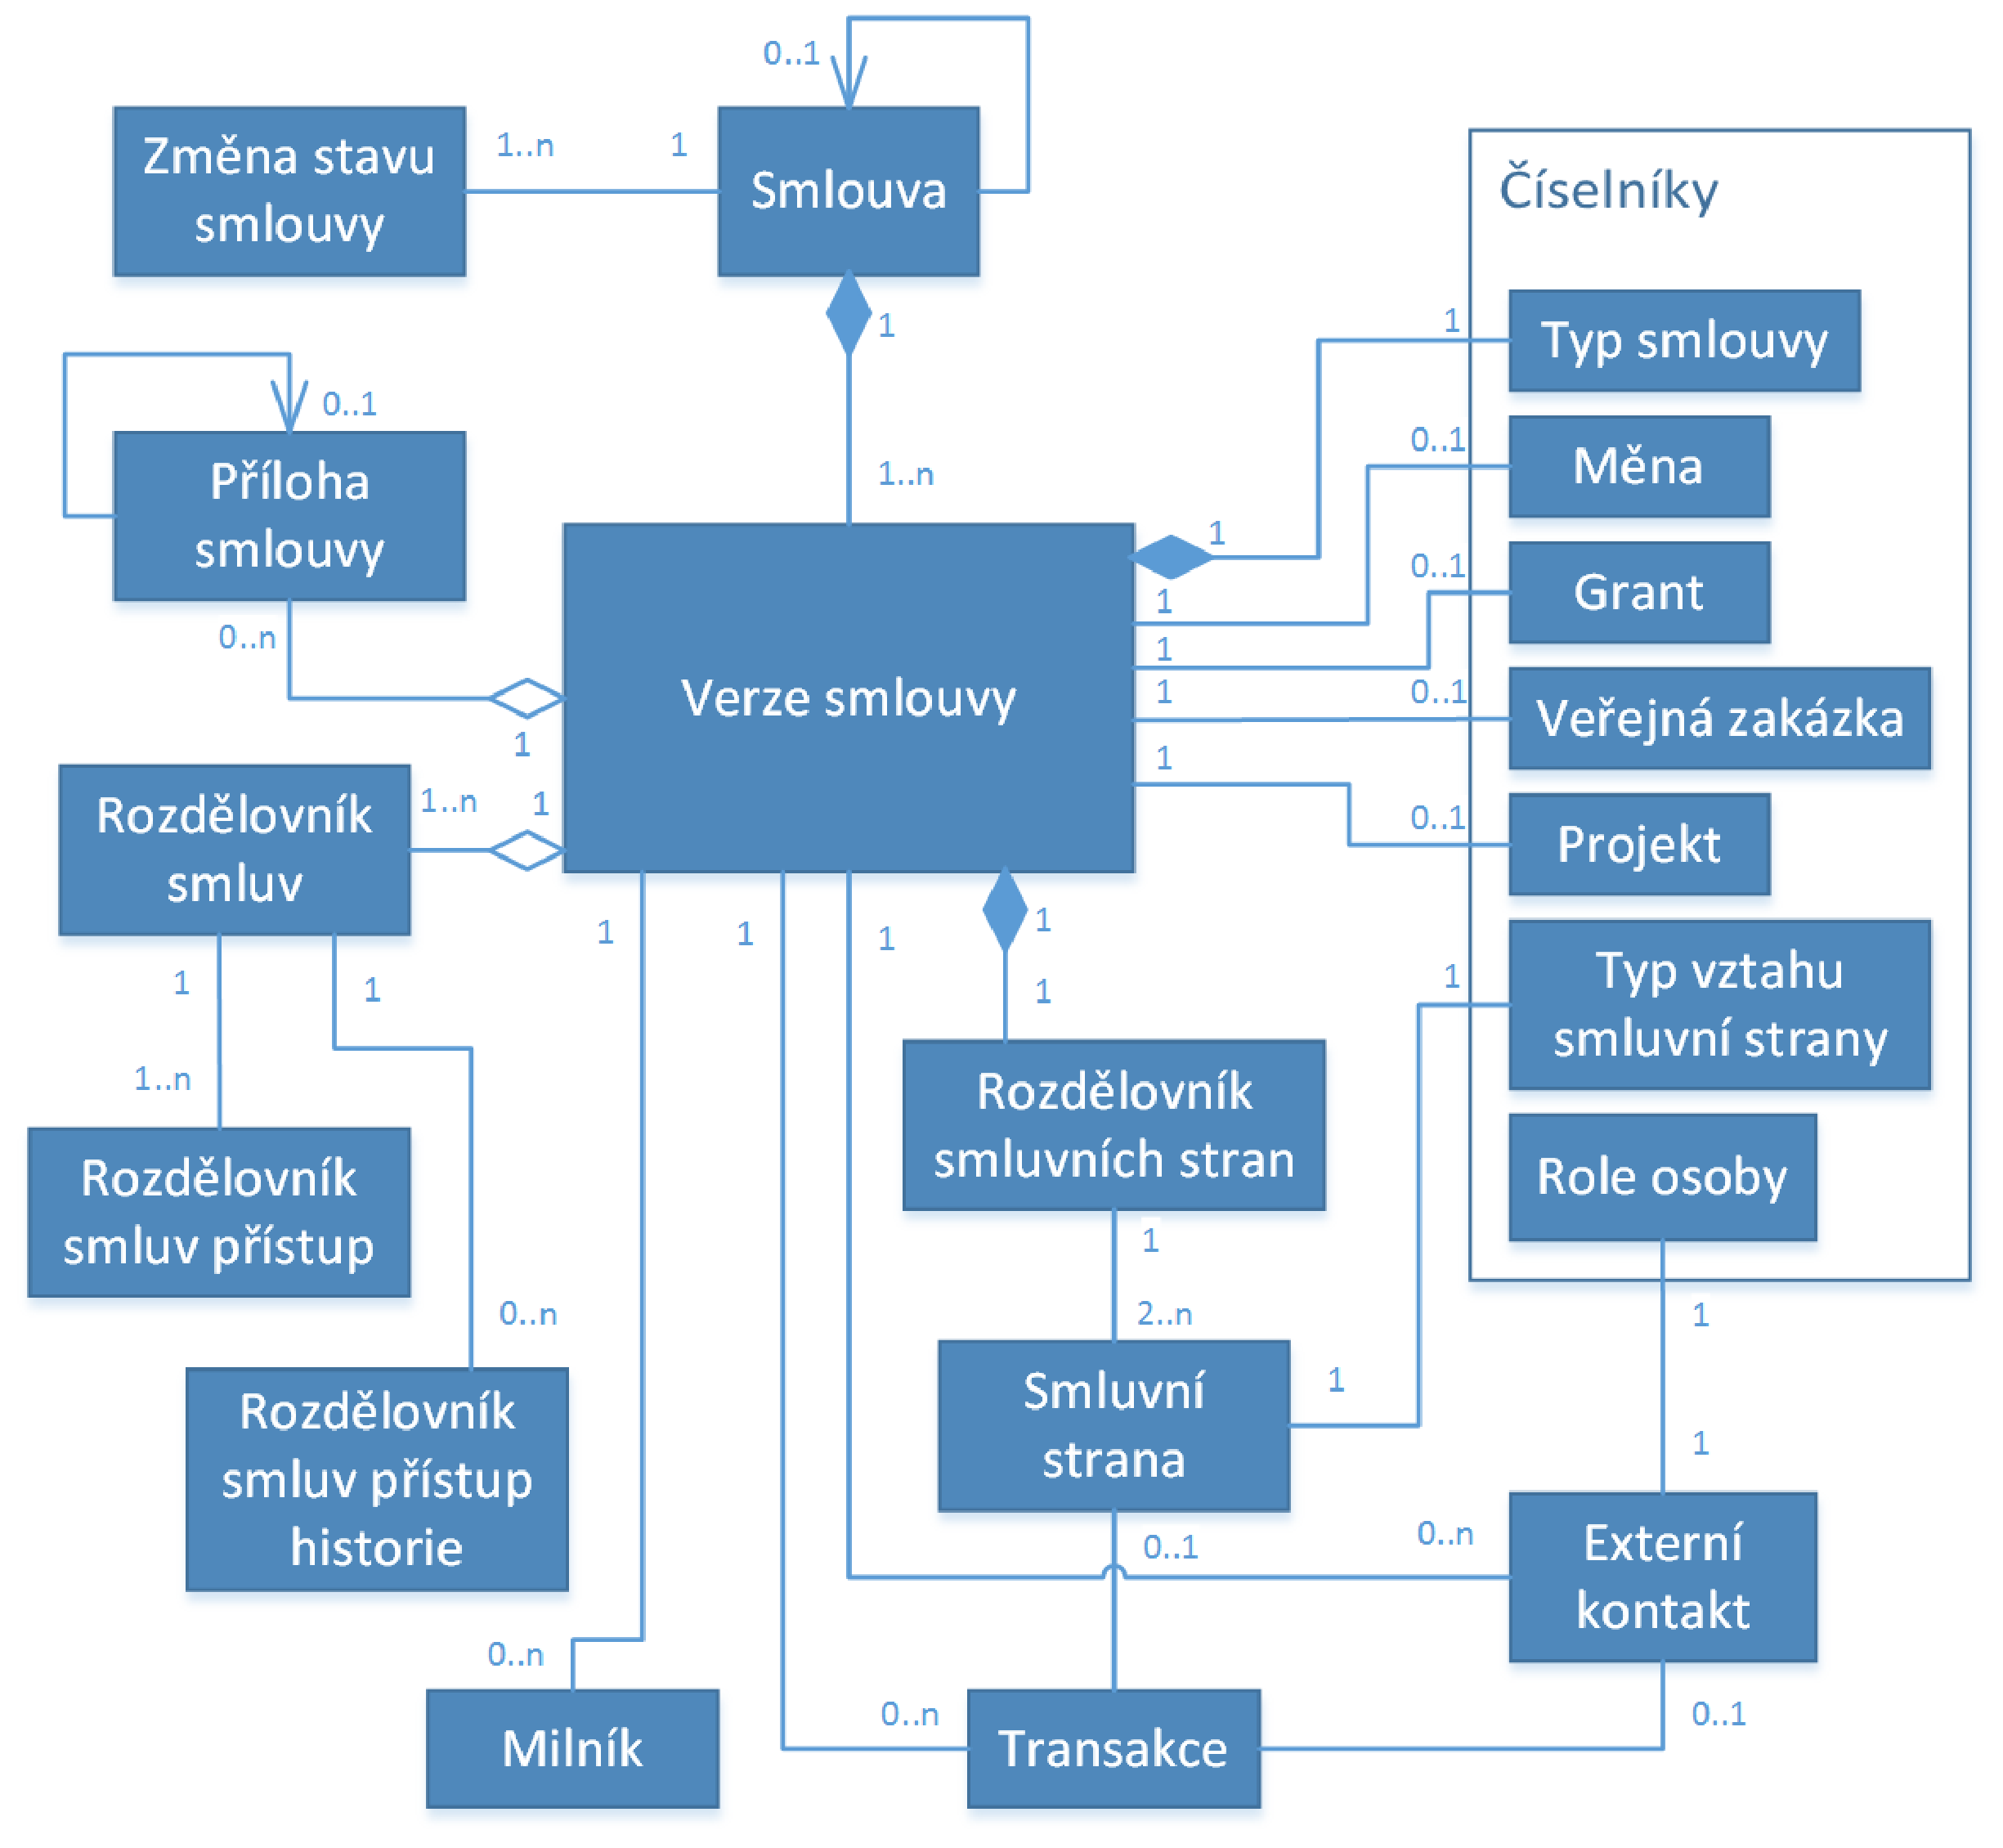
\includegraphics[width=\textwidth]{img/munisDatamodel.eps}}
\caption{ Zjednodušený datový model (bez atributů) Munis ESML}
\label{obr:munisDatamodel}
\end{figure}

\subsection{R2RML mapování}

Pomocí R2RML skriptu můžeme namapovat konkrétní sloupce z databázových tabulek na RDF predikáty. Pro složitější mapování umožňuje R2RML definovat vlastní SQL pohledy (SQL Views) nad relační databází, čehož využijeme. Pro každou entitu v rámci datového standardu proto definujeme vlastní SQL pohled. Výsledný R2RML skript lze nalézt v příloze E.

V následující části je schématicky naznačeno mapování položek. Každé entitě přiřadíme URI a typ. Následně se namapují jednotlivé položky na predikáty. Vycházíme z informací řečených v kapitole~\nameref{sec:kap4}.

\subsubsection{Smlouva}

Na obr. \ref{obr:munisSmlouva} můžeme vidět vybraný seznam tabulek a jejich atributů z datového modelu Munis ESML, které použijeme k mapování smlouvy.

\begin{figure}[H]
\centerline{\includegraphics[width=\textwidth]{img/munisSmlouva.eps}}
\caption{R2RML mapování - tabulky k mapování smlouvy}
\label{obr:munisSmlouva}
\end{figure}

Prvním krokem je přiřazení URI entitě. URI je kombinací atributu ID tabulky ESMLUV\_SMLOUVA a číslem její verze, resp. atributem PORADIVERZE tabulky (ESMLUV\_VERZESMLOUVY). Typem entity je třída cn:Contract.

\begin{itemize}
\item \textbf{URI entity} - \textit{http://[domain]/contract/\{ID\}/\{PORADIVERZE\}}
\item \textbf{Typ} - cn:Contract
\end{itemize}

\paragraph*{Konstanty}

Některé položky budou vždy obsahovat konstantní hodnotu:

\begin{itemize}
\item \textbf{dcmi:type} - s hodnotou \uv{Smlouva}
\item \textbf{cn:priceAnnual} - Nelze určit roční částku, proto vždy \uv{false}
\item \textbf{cn:funding} - Vychází zatím z nedefinovaného číselníku datového standardu, mapujeme nepovinně konstantní hodnotu \uv{vlastní}
\end{itemize}

\paragraph*{Mapované položky}

\begin{itemize}
\item \textbf{cn:anonymised} - Atribut ANONYMIZOVANO
\item \textbf{dc:title} - Atribut PREDMET
\item \textbf{dc:description} - Atribut POPIS\_POPIS
\item \textbf{dc:created} - Atribut DATUMPODPISU
\item \textbf{cn:validFrom} - Atribut DATUMUCINOSTI
\item \textbf{cn:validUntil} - Atribut DATUMUKONCENI
\item \textbf{cn:valid} - Položka je \uv{true}, jestliže se jedná o nejnovější verzi smlouvy, jinak je \uv{false}
\item \textbf{cn:contractType} - Atribut TYP, mapován na odpovídající hodnotu číselníku typů smlouvy
\item \textbf{cn:competency} - Vyplní se na základě položky TYP. Pokud je Typ smlouvy - \uv{Veřejnoprávní smlouva} vyplní se i do položky cn:competency, jinak se vyplní \uv{Soukromoprávní smlouva}
\item \textbf{cn:awardID} - Atribut EVIDENCNICISLOZAKAZKY
\item \textbf{cn:awardProfileID} - Atribut EVIDENCNICISLOFORMULARE
\item \textbf{pc:publicContract} - Atribut EVIDENCNICISLOZAKAZKY ve formě odkazu na věstník veřejných zakázek (LinkedData podoba)
	\begin{itemize}
	\item \textit{http://linked.opendata.cz/resource/domain/buyer-profiles/-\\contract/cz/\{EVIDENCNICISLOZAKAZKY\}}
	\end{itemize}
\item \textbf{cn:amount} - Odkaz na podrobné informace o ceně
	\begin{itemize}
	\item \textit{http://[domain]/contract/\{ID\}/\{PORADIVERZE\}/amount}	
	\item Mapování probíhá na objekt typu \textbf{gr:PriceSpecification} s výše zmíněným URI. Namapovány jsou položky:
		\begin{itemize}
		\item \textbf{gr:hasCurrencyValue} - Atribut CELKOVACASTKA
		\item \textbf{gr:hasCurrency} - Atribut ZKRATKA
		\end{itemize}
	\end{itemize}
\item \textbf{dc:publisher} - Odkaz na vydavatele
	\begin{itemize}
	\item \textit{http://[domain]/publisher}
	\end{itemize}
\item \textbf{cn:version} - Odkaz na informace o verzi smlouvy
	\begin{itemize}
	\item \textit{http://[domain]/contract/\{ID\}/\{PORADIVERZE\}/version}
	\end{itemize}
\item \textbf{schema:url} - Odkaz na fyzický dokument smlouvy
	\begin{itemize}
	\item \textit{http://[domain]/file/\{SADADUL\_ULOZISTEID\}/\{NAZEVSOUBORU\}}
	\end{itemize}
\item \textbf{cn:party} Odkaz na smluvní strany. Mapování probíhá skrze tabulku \\ESMLUV\_SMLSTRANROZD na které odkazují jak verze smlouvy, tak smluvní strana. Více viz R2RML skript v příloze E.
	\begin{itemize}
	\item \textit{http://[domain]/party/\{HAD\_POUZITA\}}
	\end{itemize}
\item \textbf{cn:responsiblePerson} - Každá veřejná zakázka má vazbu na externí kontakty. Externím kontaktem může být buď uživatel informačního systému (tabulka TRI\_UZIVATEL), nebo jakákoli osoba vyplněná v tabulce Externí kontakt. Pro potřeby mapování se hodnoty spojí do jednoho řetězce, viz Obr. \ref{obr:mapRespPerson}.	
\item \textbf{cn:amendment} Odkaz na dodatky. Dodatek v Munis ESML je také smlouvou, ale vždy synem jiné smlouvy nebo dodatku. Smlouvě tedy přiřadíme ty dodatky, jejichž atribut RODIC a PORADIVERZE odpovídají dané smlouvě.
	\begin{itemize}
	\item \textit{http://[domain]/amendment/\{ID\}/\{PORADIVERZE\}}
	\end{itemize}
\item \textbf{cn:attachment} Odkaz na přílohy. Každá příloha má odkaz na smlouvu (viz Obr. \ref{obr:mapAttachment})
	\begin{itemize}
	\item \textit{http://[domain]/attachment/\{ID\}/1}
	\end{itemize}
\item \textbf{cn:implementation} Odkaz na objekt Implementace
	\begin{itemize}
	\item \textit{http://[domain]/contract/\{ID\}/\{PORADIVERZE\}/implementation}
	\end{itemize}
\end{itemize}

\paragraph*{Nenamapované položky}
\begin{itemize}
\item \textbf{cn:uri} - Položka odpovídá URI entity
\item \textbf{cn:amountNoVat} - Cena bez dph, předpokládaná podpora spolu s podporou podrobného smluvního plnění
\item \textbf{cn:subjectType} - Číselník typů zboží/služeb, předpokládaná podpora u dalších verzí
\item \textbf{cn:plainText} - Prostý text dokumentu smlouvy, resp. alternativa k oskenovaným dokumentům. Vyžaduje hlubší analýzu procesu zpracování dokumentů 
\end{itemize}

\begin{figure}[H]
\centerline{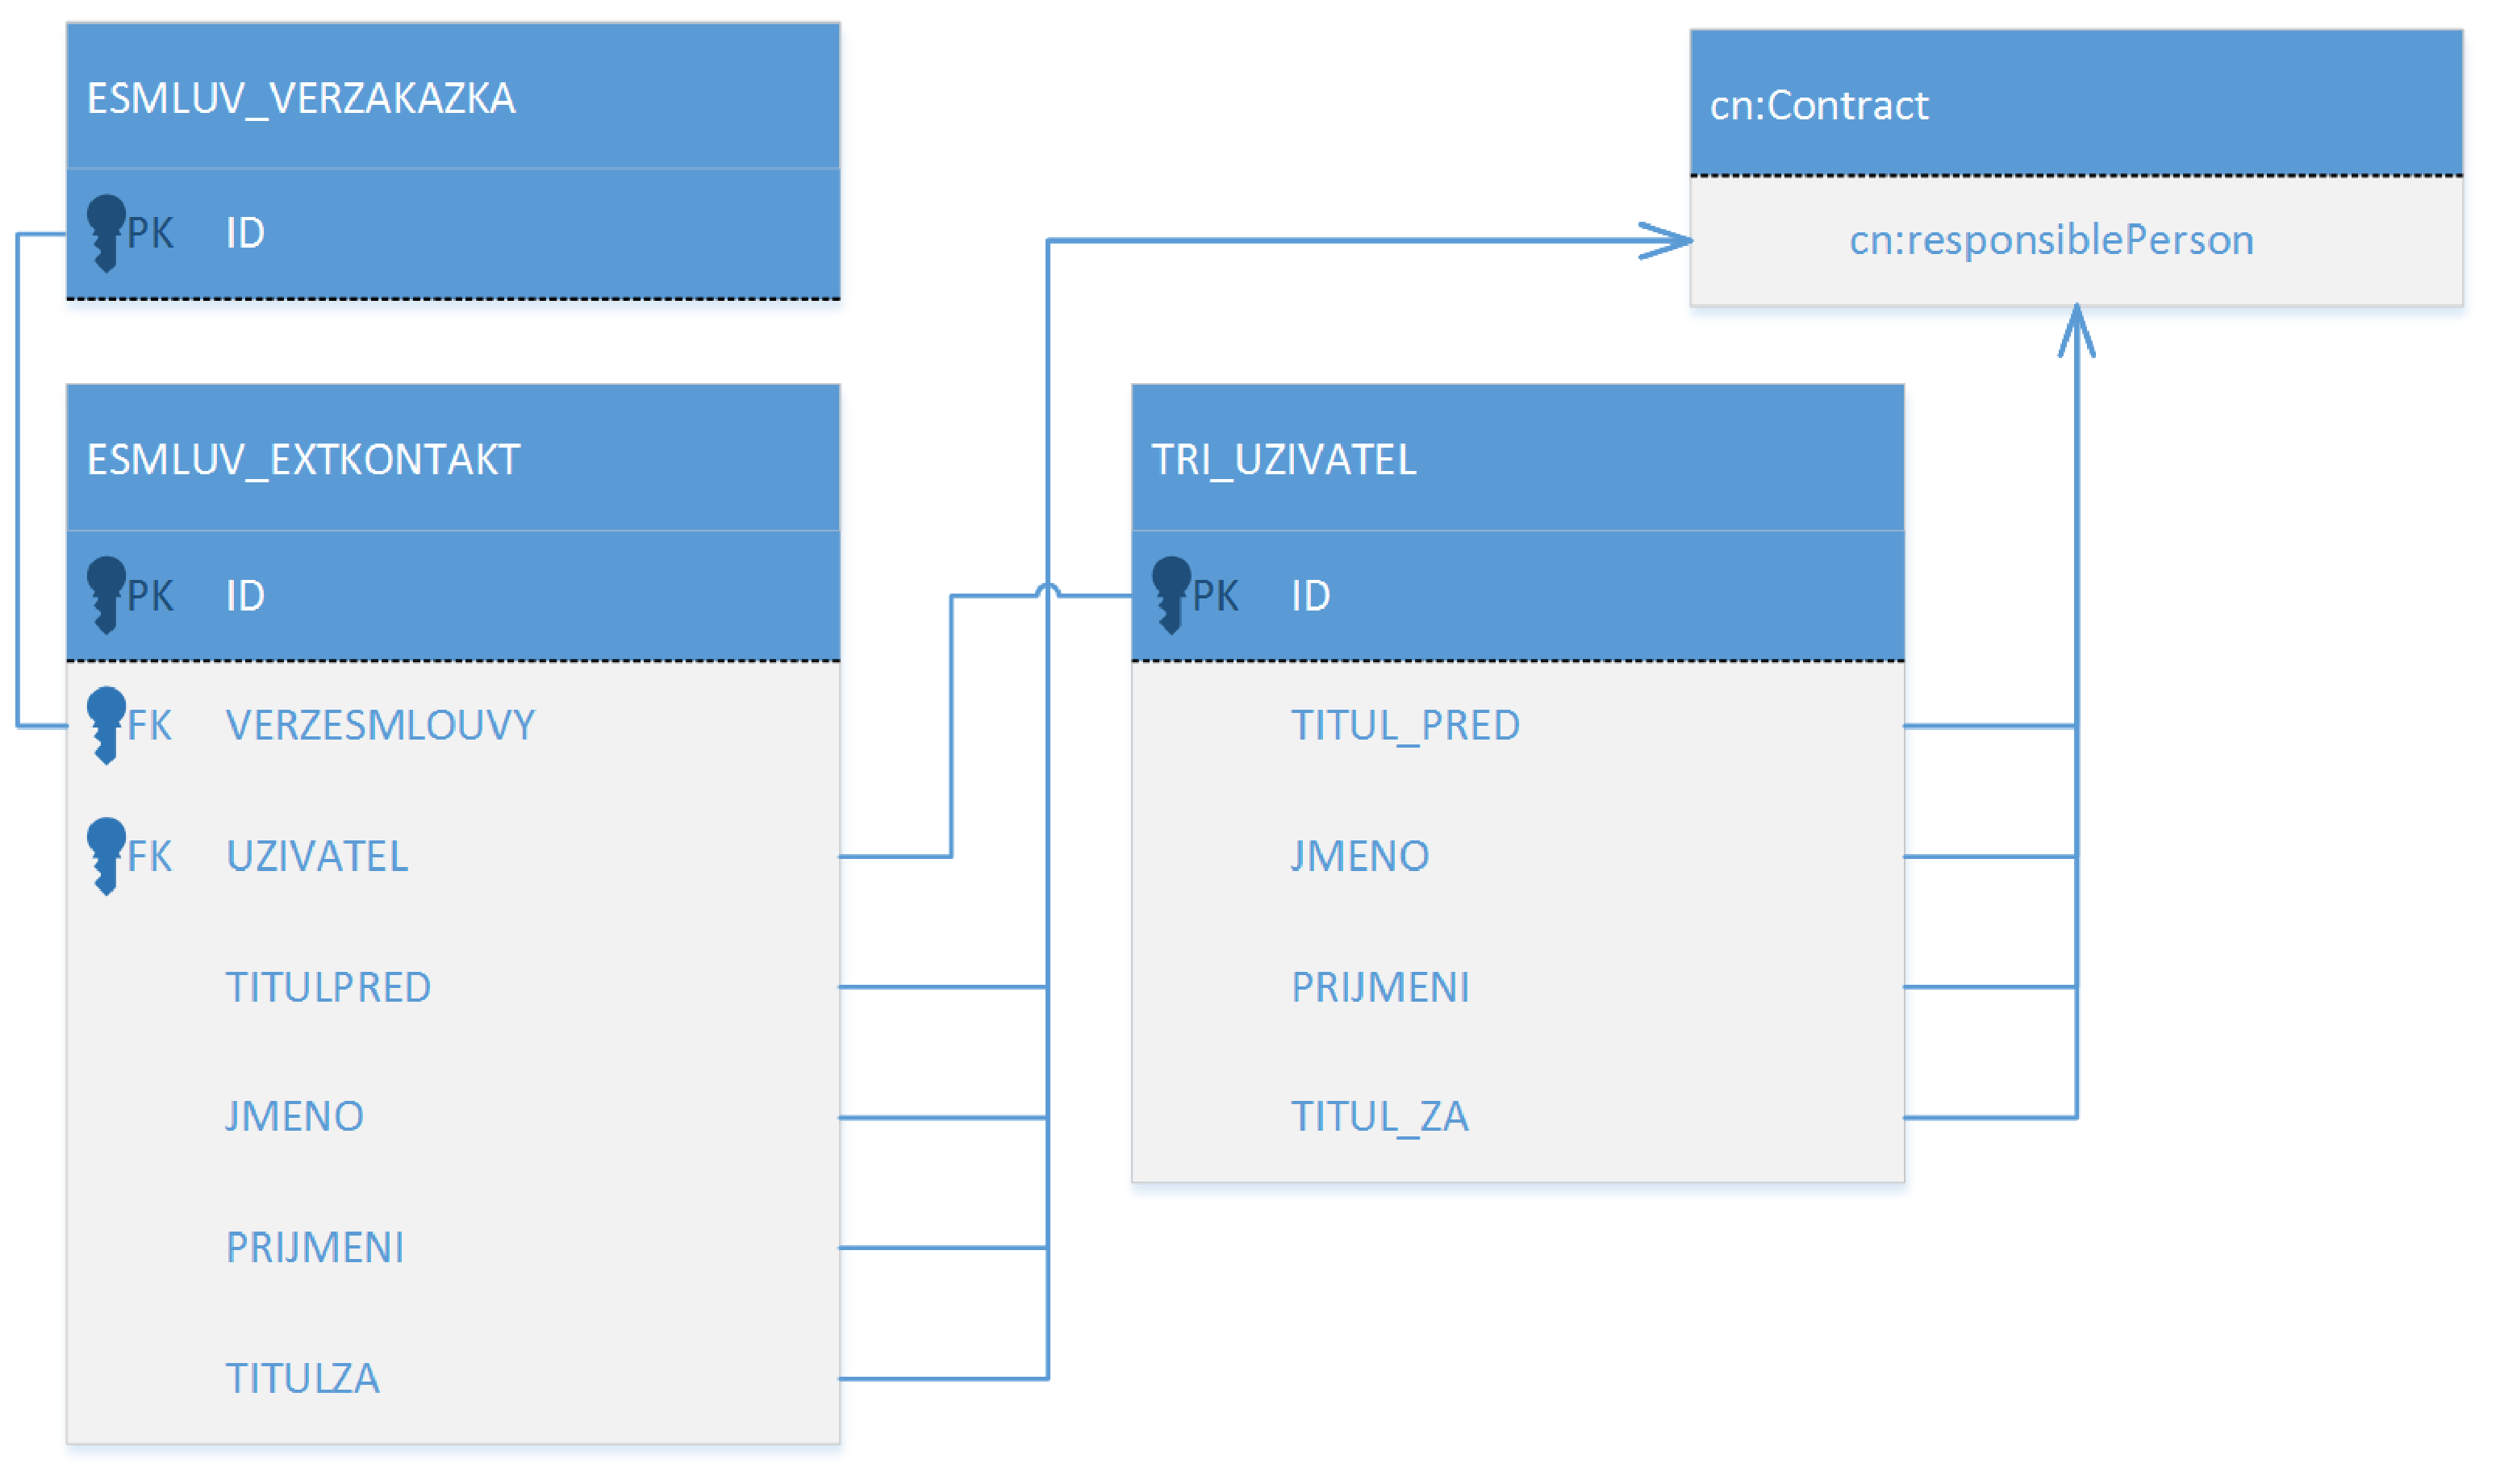
\includegraphics[width=\textwidth]{img/mapRespPerson.eps}}
\caption{R2RML mapování externího kontaktu}
\label{obr:mapRespPerson}
\end{figure}

\subsubsection{Smluvní strana}

Mapování smluvní strany a adresy vychází z údajů tabulek \\ESMLUV\_SMLUVSTRANA a HAD\_POUZITA (viz Obr. \ref{obr:mapParty})

\begin{itemize}
\item \textbf{URI} - \textit{http://[domain]/party/\{HAD\_POUZITA\}}
\item \textbf{Typ} - gr:BusinessEntity
\end{itemize}

\paragraph*{Mapované položky}
\begin{itemize}
\item \textbf{gr:legalName} - Atribut NAZEV\_SUBJEKTU
\item \textbf{dc:identifier} - Atribut ICO
\item \textbf{owl:sameAs} - Atribut ICO, odkaz na reprezentaci ekonomického subjektu v ARESu (LinkedData podoba)
	\begin{itemize}
	\item \textit{http://linked.opendata.cz/resource/business-entity/CZ\{ICO\}}
	\end{itemize}
\item \textbf{cn:noID} - \uv{true} pokud je vyplněno IČ, jinak \uv{false}
\item \textbf{cn:localID} - Atribut HAD\_POUZITA
\item \textbf{schema:addressCountry} - Atribut STAT
\item \textbf{cn:paysVAT} - Atribut PLATCEDPH
\item \textbf{schema:address} - Odkaz na adresu
	\begin{itemize}
	\item \textit{http://[domain]/party/\{HAD\_POUZITA\}/address}
	\end{itemize}
\end{itemize}

\paragraph*{Nenamapované položky}
\begin{itemize}
\item \textbf{cn:payer} - Modul ESML zatím neeviduje kompletní smluvní plnění, takže nelze určit 
\item \textbf{cn:superiorInstitution} - Modul ESML neeviduje nadřazené instituce
\end{itemize}

\subsubsection{Adresa}

\begin{itemize}
\item \textbf{URI} - \textit{http://[domain]/party/{HAD\_POUZITA}/address}
\item \textbf{Typ} - schema:PostalAddress
\end{itemize}

\paragraph*{Mapované položky}
\begin{itemize}
\item \textbf{schema:streetAddres} - Složení atributu ULICE a CISLA
\item \textbf{schema:postalCode} - Atribut PSC
\item \textbf{schema:addressLocality} - Atribut MESTO
\end{itemize}

\paragraph*{Nenamapované položky}
\begin{itemize}
\item \textbf{cn:nuts} - Modul ESML neeviduje hodnoty normalizované klasifikace územních celků
\end{itemize}

\begin{figure}[H]
\centerline{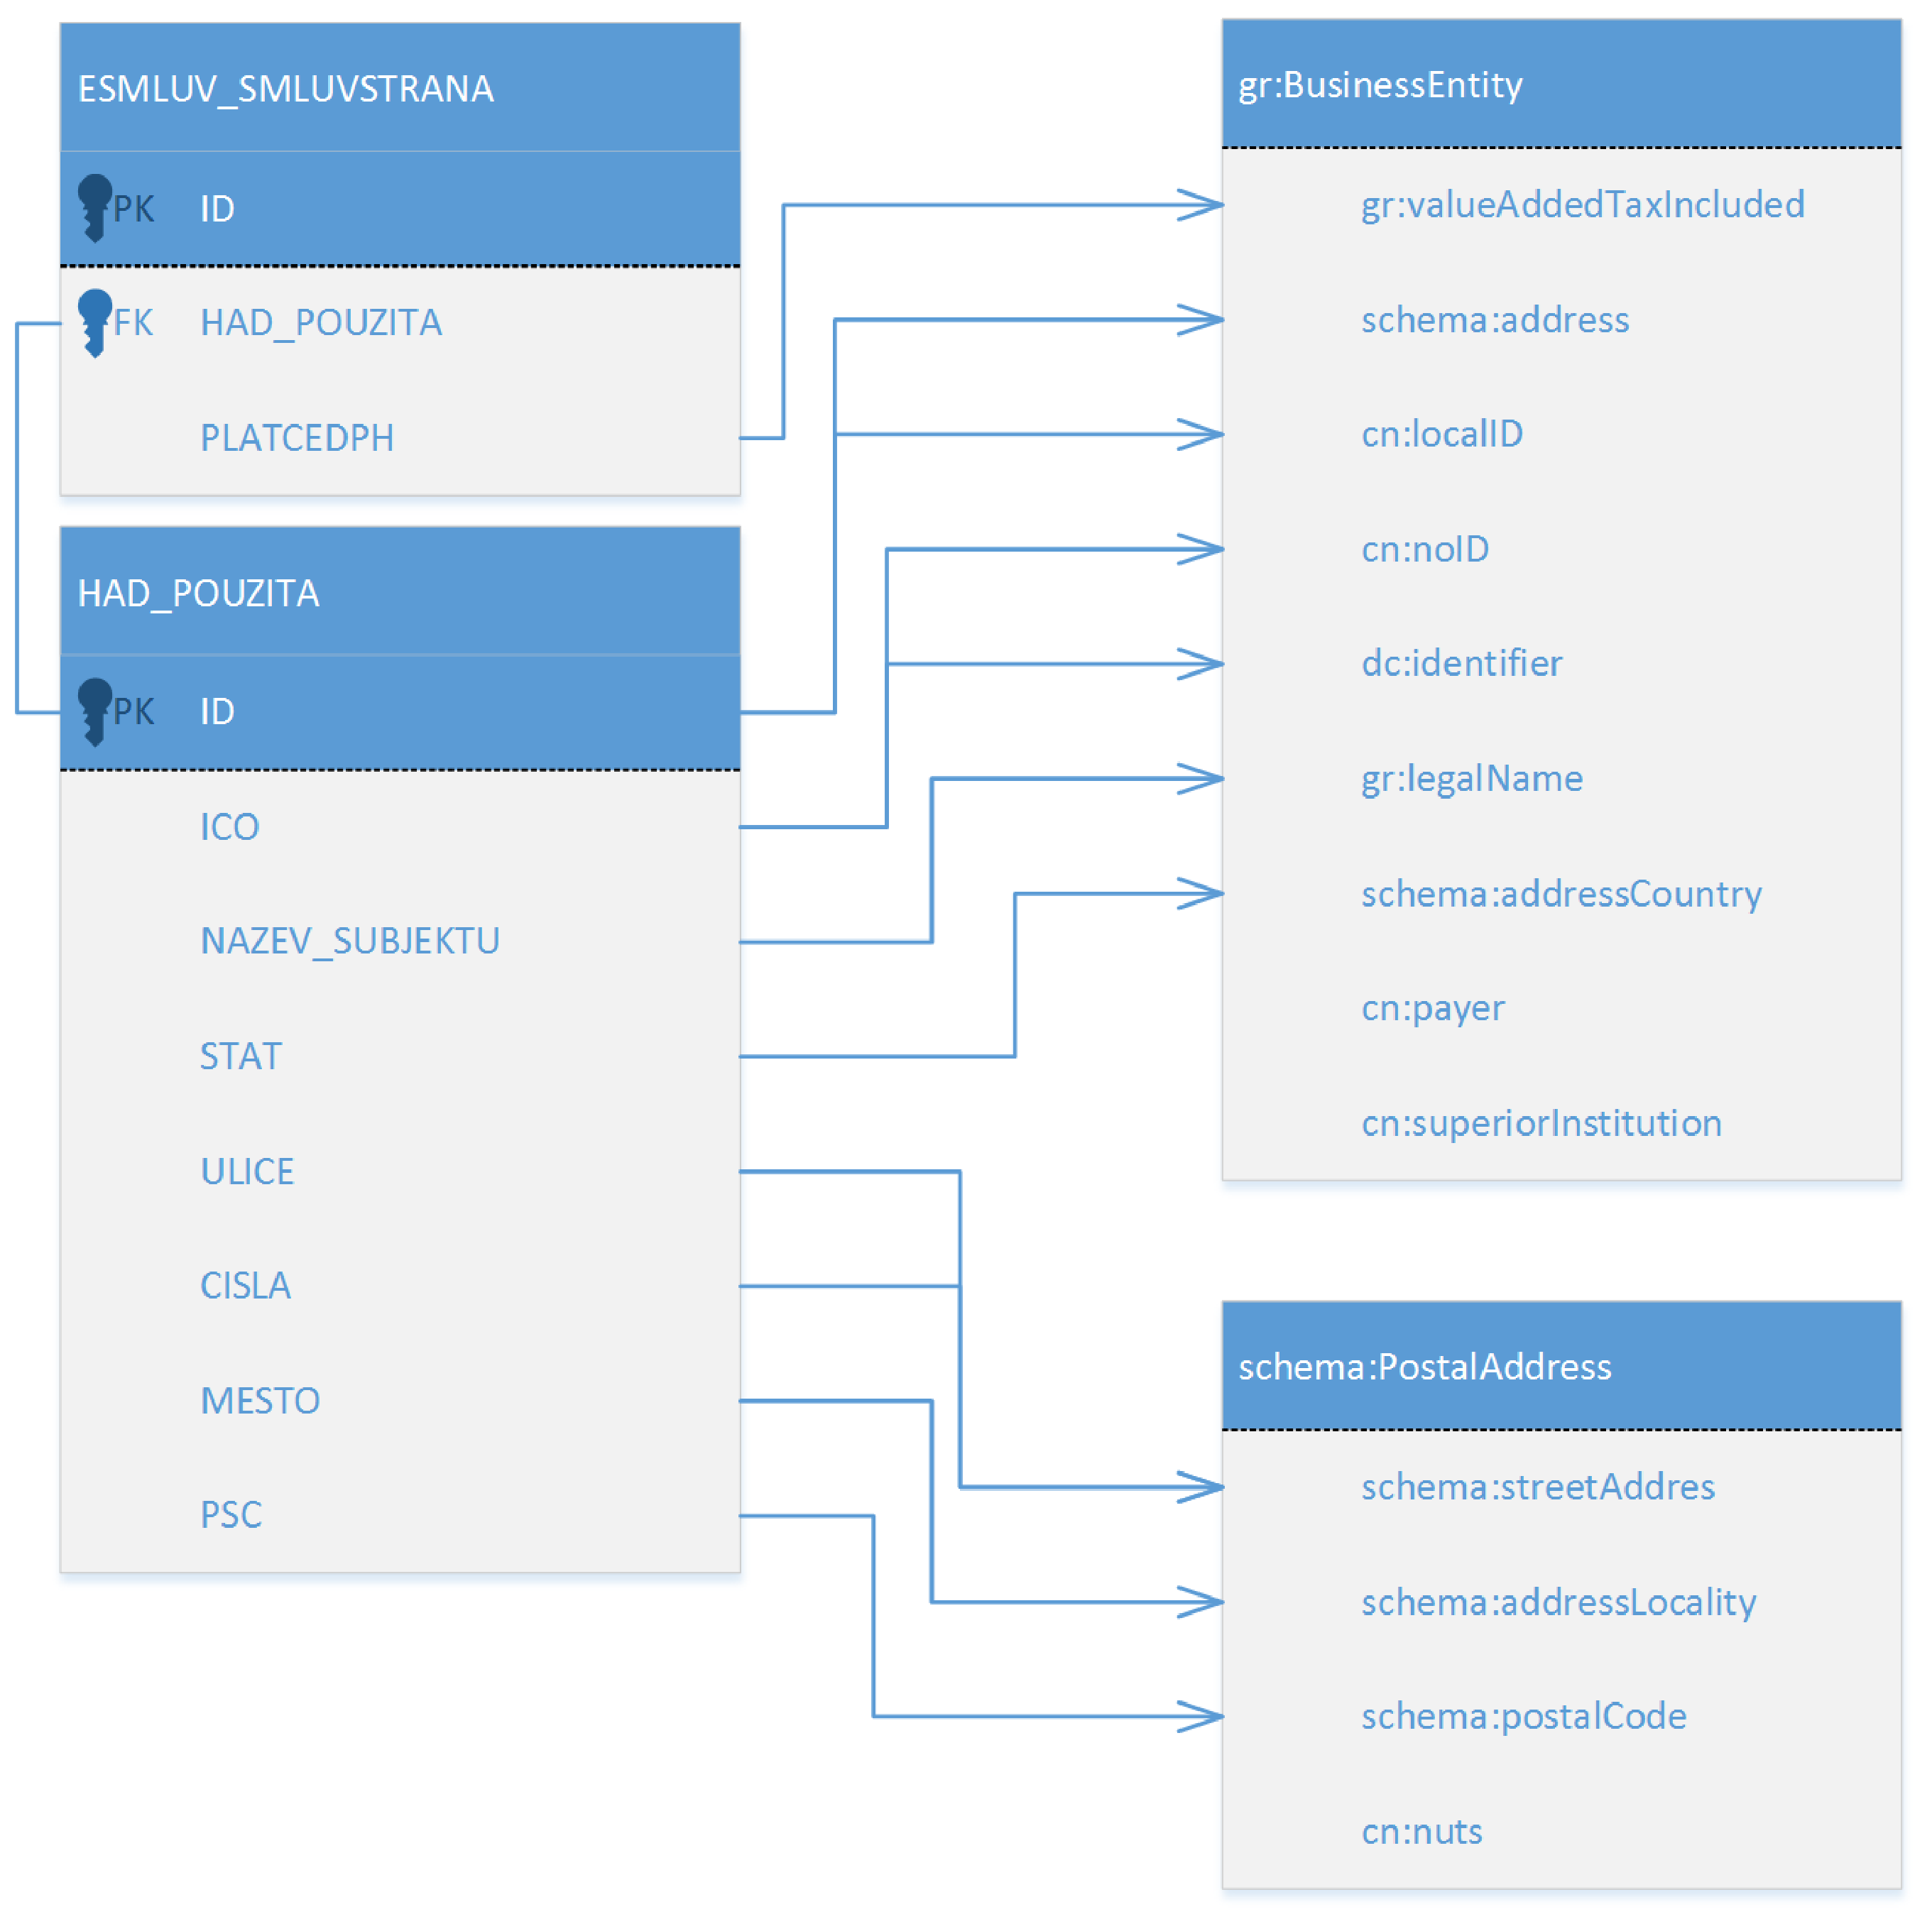
\includegraphics[width=\textwidth]{img/mapParty.eps}}
\caption{R2RML mapování vlastností Smluvní strany a Adresy}
\label{obr:mapParty}
\end{figure}

\subsubsection{Příloha}

Mapování přílohy vychází z údajů tabuly \\ESMLUV\_PRILOHASMLOUVY (viz Obr. \ref{obr:mapAttachment}). V modulu smluv lze přílohy editovat, ale neprovádí se jejich verzování. Proto verze přílohy bude mít vždy hodnotu \uv{1}. Oproti datovému standardu, příloha v datovém modelu Munis ESML popisuje spíše fyzický soubor, nemůžeme tedy namapovat většinu položek entity Dokument, ale jen některé. Nemapované položky proto neuvádíme.

\begin{itemize}
\item \textbf{URI} entity  - \textit{http://[domain]/attachment/\{ID\}/1}
\item \textbf{Typ} - cn:Attachment
\end{itemize}

\paragraph*{Konstanty}
\begin{itemize}
\item \textbf{dcmi:type} - Hodnota \uv{Příloha}
\item \textbf{cn:valid} - Položka je vždy \uv{true}, přílohy nejsou verzované
\end{itemize}

\paragraph*{Mapované položky}
\begin{itemize}
\item \textbf{cn:anonymised} - Atribut ANONYMIZOVANO
\item \textbf{dc:title} - Atribut POPIS\_NAZEV
\item \textbf{dc:identifier} - Atribut ID
\item \textbf{schema:url} - Odkaz na fyzické umístění souboru
	\begin{itemize}
	\item \textit{http://[domain]/file/\{SADADUL\_ULOZISTEID\}/\{NAZEVSOUBORU\}}
	\end{itemize}
\item \textbf{dc:publisher} - Odkaz na vydavatele
	\begin{itemize}
	\item \textit{http://[domain]/publisher}
	\end{itemize}
\item \textbf{cn:version} - Odkaz na informace o verzi smlouvy
	\begin{itemize}
	\item \textit{http://[domain]/attachment/{ID}/1/version}
	\end{itemize}
\item \textbf{cn:contract} - Odkaz na nadřízenou smlouvu. K tomuto údaji je třeba ID Smlouvy (tabulka ESMLUV\_SMLOUVA a pořadí verze smlouvy, tabulka ESMLUV\_VERZESMLOUVY)
	\begin{itemize}
	\item \textit{http://[domain]/attachment/\{ID\}/\{PORADIVERZE\}}
	\end{itemize}
\end{itemize}

\begin{figure}[H]
\centerline{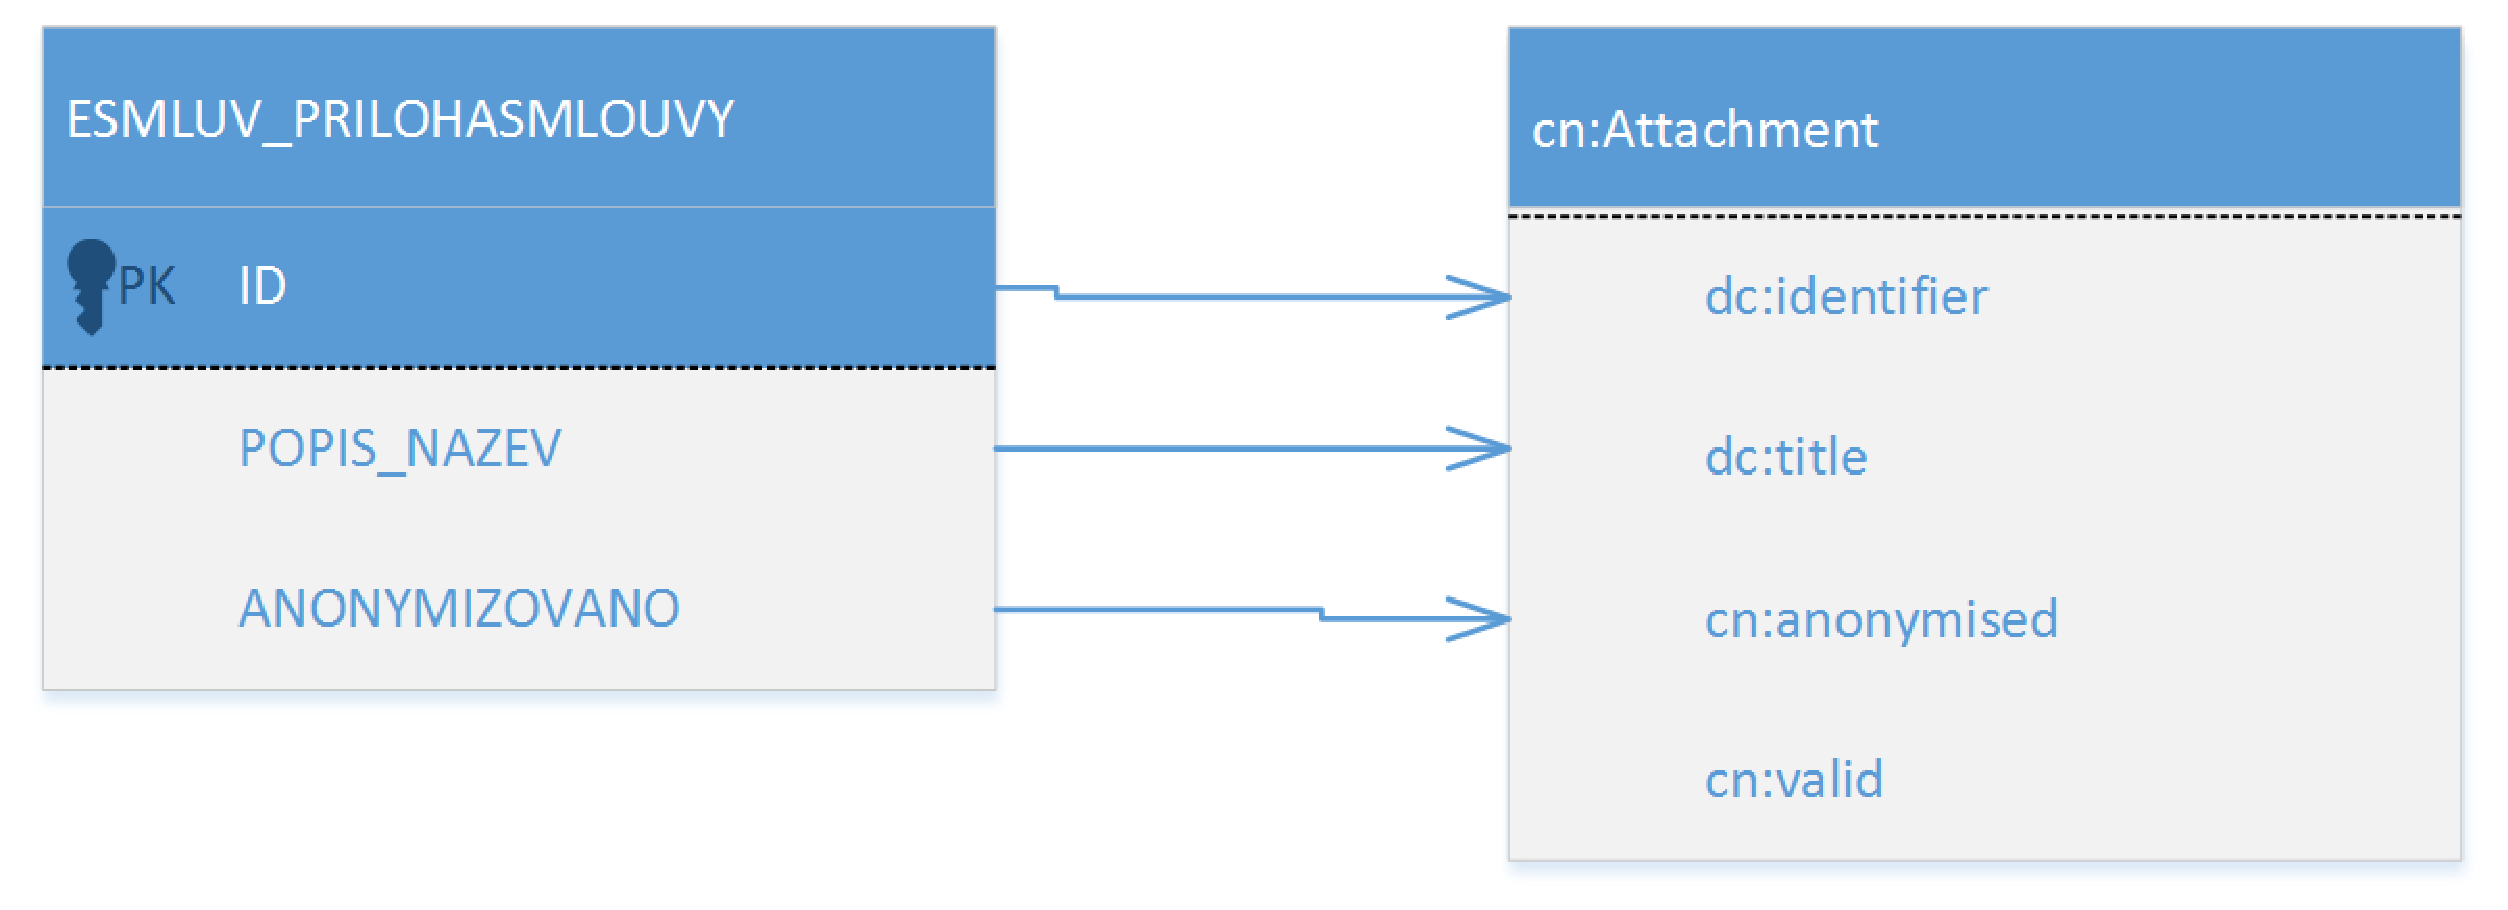
\includegraphics[width=\textwidth]{img/mapAttachment.eps}}
\caption{R2RML mapování vlastností Příloha}
\label{obr:mapAttachment}
\end{figure}

\subsubsection{Dodatek}

Dodatek v datovém modelu Munis ESML je také smlouvou, takže budeme vycházet z atributů jako u smlouvy (viz Obr. \ref{obr:munisSmlouva}).

\begin{itemize}
\item \textbf{URI entity} - \textit{http://[domain]/amendment/{ID}/{PoradiVerzeDodatku}}
\item \textbf{Typ} - cn:Amendment
\end{itemize}

\paragraph*{Konstanty}

\begin{itemize}
\item \textbf{dcmi:type} - s hodnotou \uv{Dodatek}
\end{itemize}

\paragraph*{Mapované položky}

\begin{itemize}
\item \textbf{cn:anonymised} - Atribut ANONYMIZOVANO
\item \textbf{dc:title} - Atribut PREDMET
\item \textbf{dc:identifier} - Atribut ID
\item \textbf{dc:created} - Atribut DATUMPODPISU
\item \textbf{cn:valid} - Položka je \uv{true}, jestliže se jedná o nejnovější verzi dodatku, jinak je \uv{false}
\item \textbf{cn:contract} - Odkaz rodičovskou smlouvu
	\begin{itemize}
	\item \textit{http://[domain]/contract/\{RODIC\}/\{PORADIVERZE\}}
	\end{itemize}
\item \textbf{dc:publisher} - Odkaz na vydavatele
	\begin{itemize}
	\item \textit{http://[domain]/publisher}
	\end{itemize}
\item \textbf{cn:version} - Odkaz na informace o verzi dodatku
	\begin{itemize}
	\item \textit{http://[domain]/contract/\{ID\}/\{PORADIVERZE\}/version}
	\end{itemize}
\item \textbf{schema:url} - Odkaz na fyzický dokument dodatku
	\begin{itemize}
	\item \textit{http://[domain]/file/\{SADADUL\_ULOZISTEID\}/\{NAZEVSOUBORU\}}
	\end{itemize}
\item \textbf{cn:responsiblePerson} - Každá veřejná zakázka má vazbu na externí kontakty. Externím kontaktem může být buď uživatel informačního systému (tabulka TRI\_UZIVATEL), nebo jakákoli osoba vyplněná v tabulce Externí kontakt. Pro potřeby mapování se hodnoty spojí do jednoho řetězce, viz Obr. \ref{obr:mapRespPerson}.
\end{itemize}

\paragraph*{Nenamapované položky}
\begin{itemize}
\item \textbf{cn:uri} - Položka odpovídá URI entity
\item \textbf{cn:plainText} - Prostý text dokumentu smlouvy, resp. alternativa k oskenovaným dokumentům. Vyžaduje hlubší analýzu procesu zpracování dokumentů 
\end{itemize}

\subsubsection{Verze dokumentu}

K mapování jednotlivých verzí smlouvy/přílohy/dodatku. Pro smlouvy/dodatky mapujeme z tabulky ESMLUV\_VERZESMLOUVY (viz Obr. \ref{obr:mapVersion}). Pro přílohu mapujeme z tabulky ESMLUV\_PRILOHA (viz. Obr. \ref{obr:mapAttachment})

\begin{itemize}
\item \textbf{URI entity}
	\begin{itemize}
	\item U smlouvy/dodatku - \\\textit{http://[domain]/[type]/\{ID\}/\{PORADIVERZE\}/version}
	\item U přílohy - \textit{http://[domain]/attachment/\{ID\}/1/version}
	\end{itemize}
\item \textbf{Typ} - cn:Version
\end{itemize}

\paragraph*{Mapované položky}
\begin{itemize}
\item \textbf{cn:uri} - Položka je stejná jako URI entity
\item \textbf{cn:versionOrder} - U smlouvy/dodatku atribut PORADIVERZE, u přílohy hodnota \uv{1}
\item \textbf{dc:issued} - U smlouvy/dodatku atribut DATUMZMENYSTAVU\_TS, u přílohy hodnota OKAMZIKVYTVORENI
\end{itemize}

\paragraph*{Nenamapované položky}
\begin{itemize}
\item \textbf{cn:publisherId} - Díky Id a verzi dokumentu máme každou entitu jednoznačně identifikovanou, proto není třeba vyplňovat.
\end{itemize}

\begin{figure}[H]
\centerline{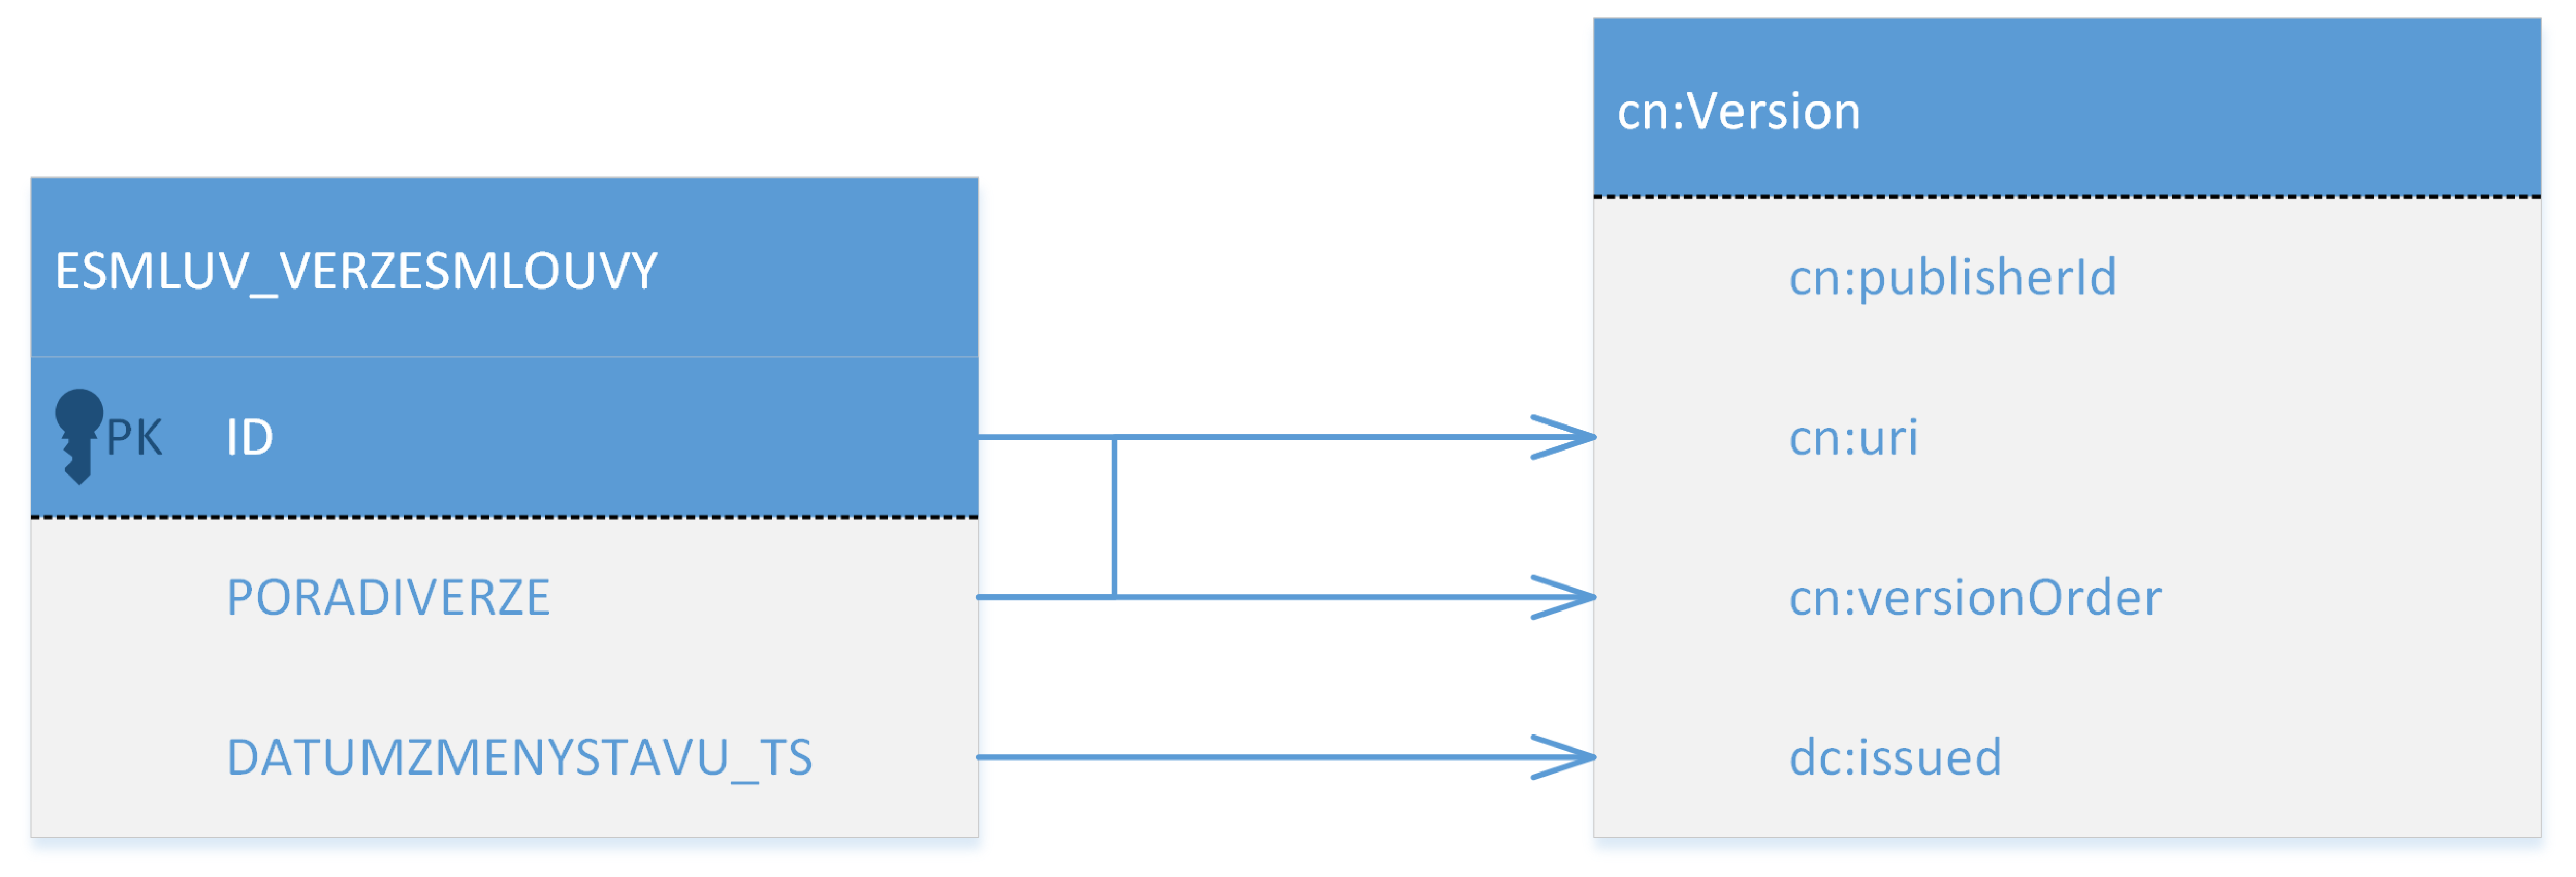
\includegraphics[width=\textwidth]{img/mapVersion.eps}}
\caption{R2RML mapování vlastností Verze}
\label{obr:mapVersion}
\end{figure}

\subsubsection{Implementace}

Entitu implementace nereprezentuje žádná tabulka v rámci datového modulu ERMS. Je třeba ji proto vytvořit s odpovídajícími položkami. Využijeme tabulek ESMLUV\_SMLOUVA, ESMLUV\_VERZESMLOUVY a ESMLUV\_MILNIK. 

\begin{itemize}
\item \textbf{URI entity} - \textit{http://[domain]/contract/{ID}/{PORADIVERZE}/implementation}
\item \textbf{Typ} - cn:Implementation
\end{itemize}

\paragraph*{Mapované položky}
\begin{itemize}
\item \textbf{cn:milestone} - Položka je stejná jako URI entity
	\begin{itemize}
	\item textit{http://[domain]/contract/\{ID\}/\{PORADIVERZE\}/milestone/- \{MilestoneID\}}
	\end{itemize}
\end{itemize}

\subsubsection{Milník}

K mapování milníků využijeme tabulek ESMLUV\_SMLOUVA, \\ESMLUV\_VERZESMLOUVY a ESMLUV\_MILNIK (tabulka milníku viz Obr. \ref{obr:mapMilestone}).

\begin{itemize}
\item \textbf{URI entity} - \textit{http://[domain]/contract/\{ID\}/\{PORADIVERZE\}/milestone/-
\{MilestoneID\}}
\item \textbf{Typ} - cn:Milestone
\end{itemize}

\paragraph*{Mapované položky}
\begin{itemize}
\item \textbf{dc:title} - Atribut NAZEV
\item \textbf{cn:dueDate} - Atribut DATUMUCINOSTIML
\end{itemize}

\begin{figure}[H]
\centerline{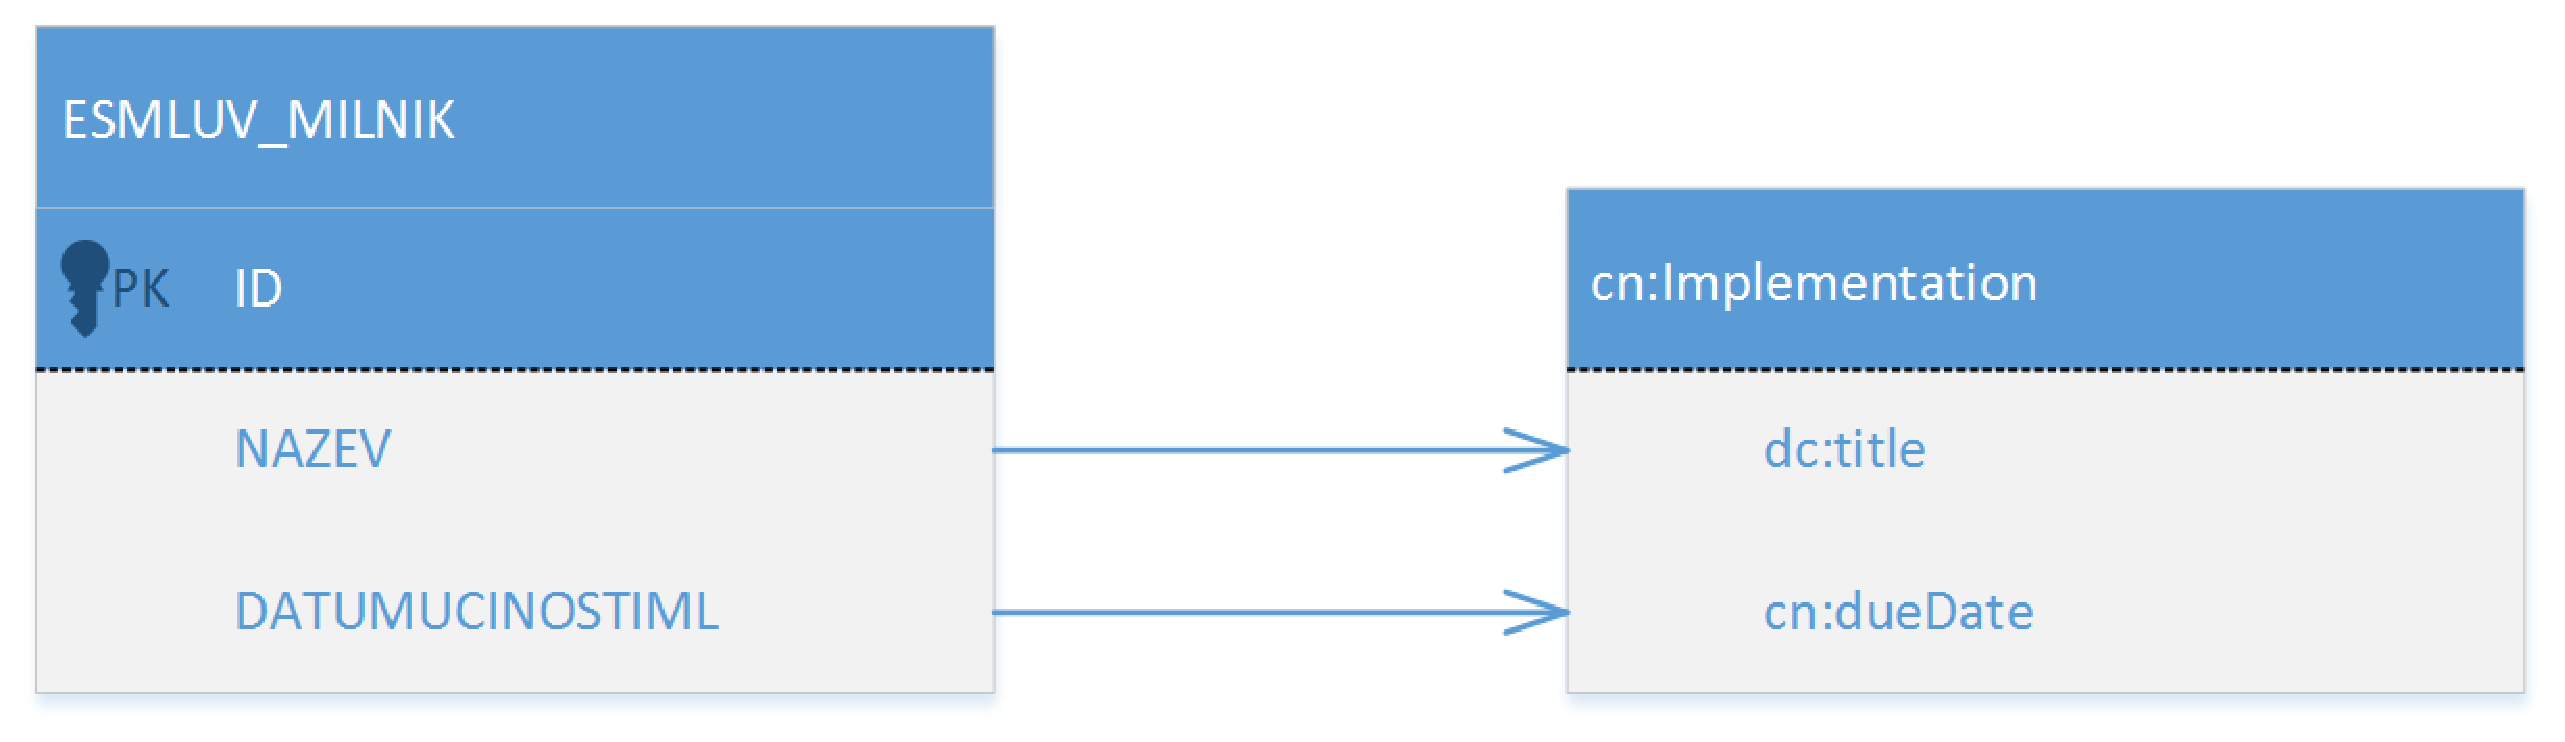
\includegraphics[width=\textwidth]{img/mapMilestone.eps}}
\caption{R2RML mapování vlastností Milníku}
\label{obr:mapMilestone}
\end{figure}

\subsubsection{Vydavatel}

Vydavatele namapujeme pomocí tabulky TRI\_ORGADR, viz Obr. \ref{obr:mapPublisher}

\begin{itemize}
\item \textbf{URI entity}  - \textit{http://[domain]/publisher}
\item \textbf{Typ} - foaf:Organization
\end{itemize}

\paragraph*{Konstanty}
\begin{itemize}
\item \textbf{schema:addressCountry} - Hodnota \uv{CZE}
\end{itemize}

\paragraph*{Mapované položky}
\begin{itemize}
\item \textbf{gr:legalName} - Atribut NAZEVORGANIZACE
\item \textbf{cn:noID} - \uv{true} pokud je vyplněno IČ, jinak \uv{false}
\item \textbf{dc:identifier} - Atribut ICO
\item \textbf{owl:sameAs} - Atribut ICO, odkaz na reprezentaci ekonomického subjektu v ARESu (LinkedData podoba)
	\begin{itemize}
	\item \textit{http://linked.opendata.cz/resource/business-entity/CZ\{ICO\}}
	\end{itemize}
\end{itemize}

\paragraph*{Nenamapované položky}
\begin{itemize}
\item \textbf{cn:authentication} - Pro naše účely nemá smysl
\end{itemize}

\begin{figure}[H]
\centerline{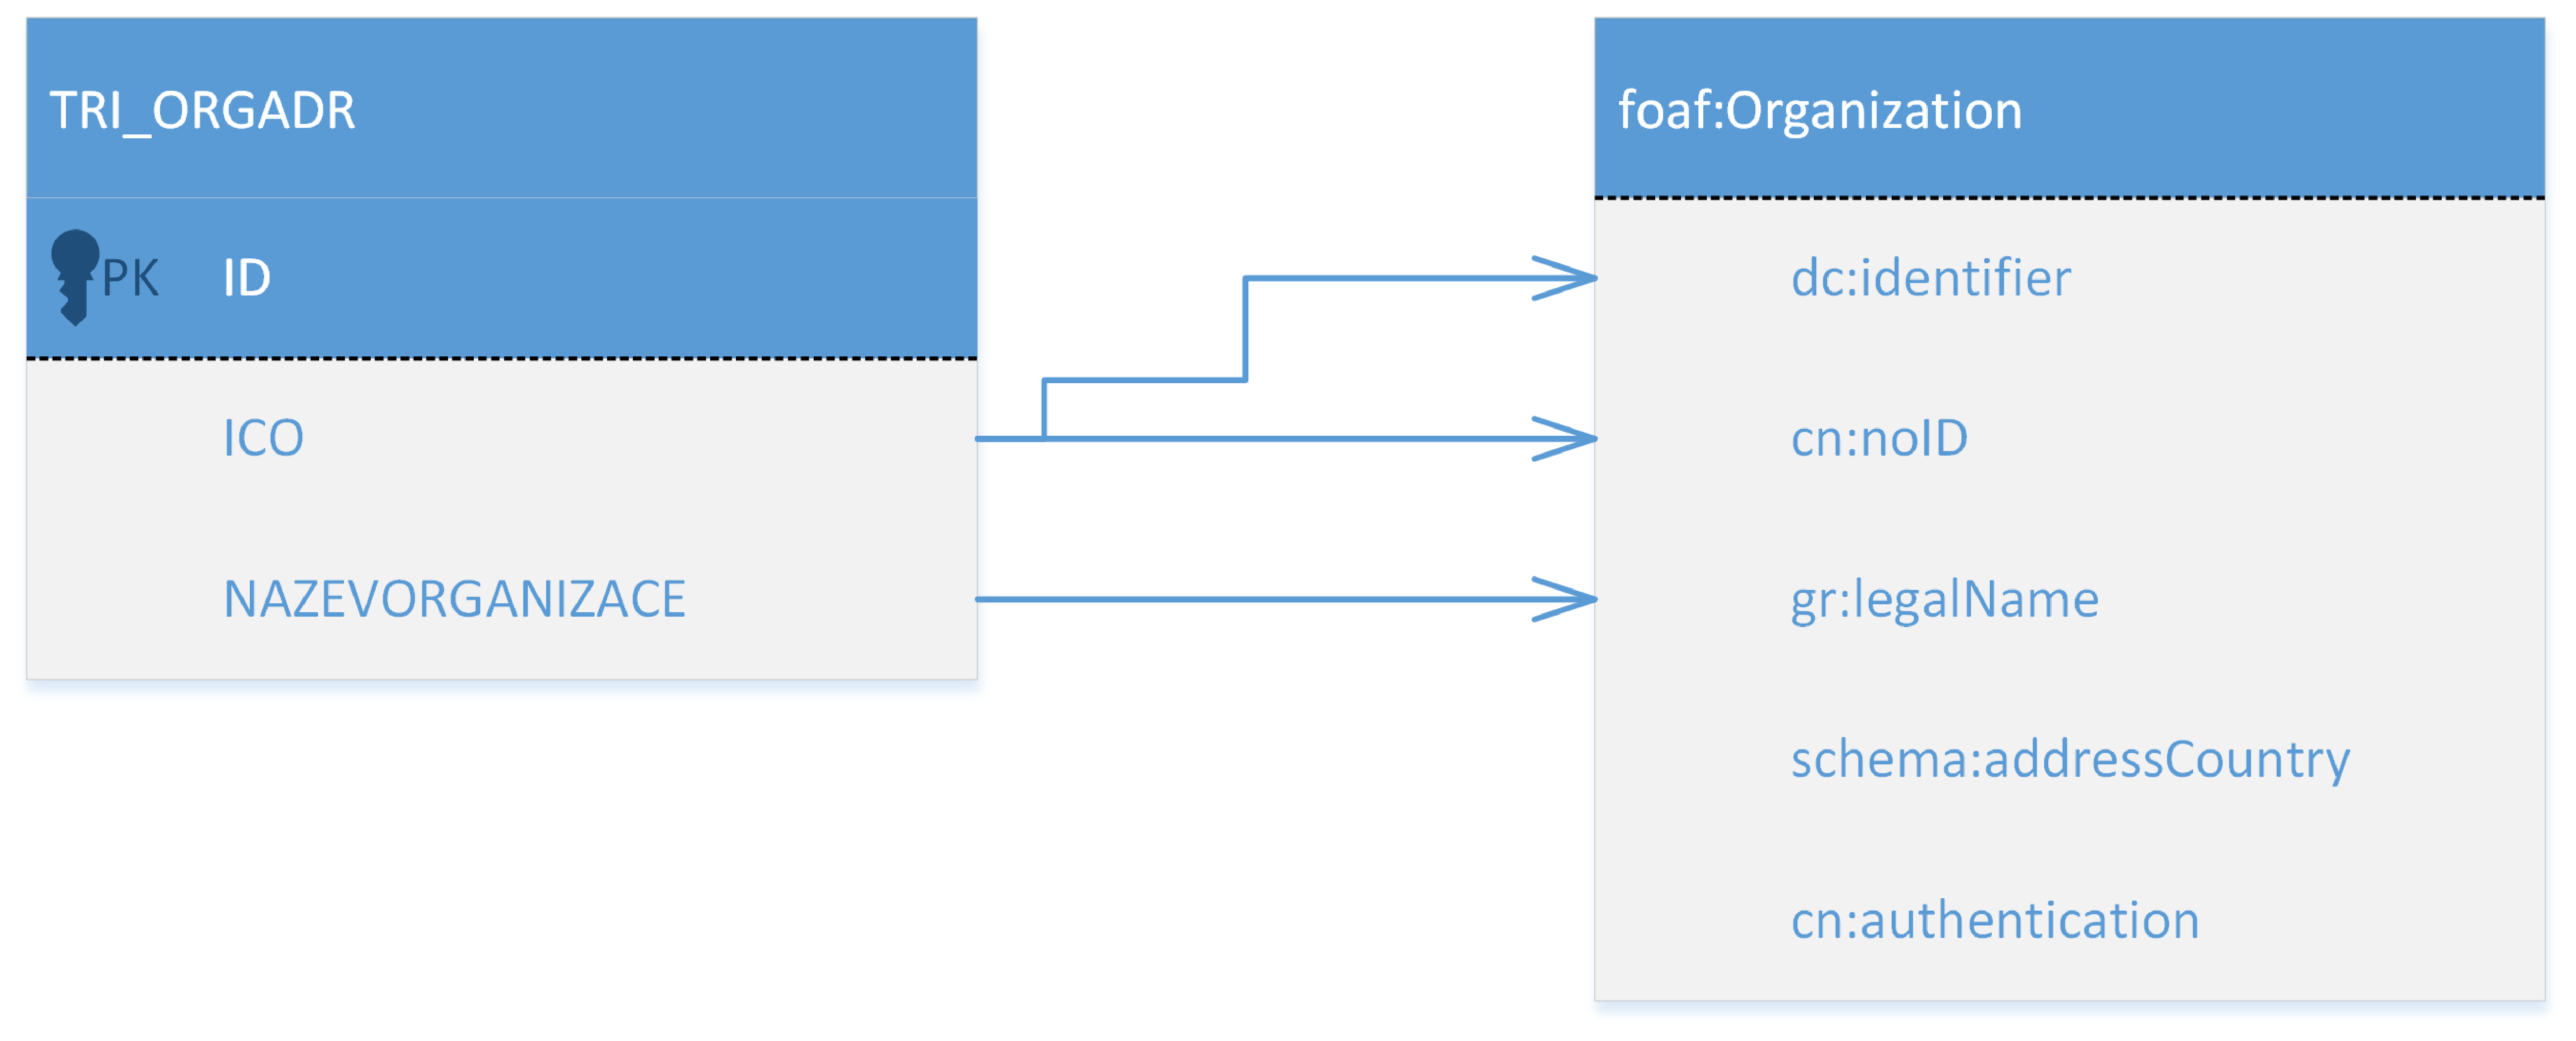
\includegraphics[width=\textwidth]{img/mapPublisher.eps}}
\caption{R2RML mapování vlastností Vydavatele}
\label{obr:mapPublisher}
\end{figure}

\subsection{Volba technologií a implementační platformy}

Pro samotnou implementaci konverzního mechanismu zvolíme platformu .Net. Modul bude mít formu webové aplikace, resp. virtuálního SPARQL endpointu, kterou budeme implementovat v technologii ASP.Net. Využijeme tradičního architektonického vzoru MVC. K práci s RDF daty budeme využívat knihovnu dotnetRdf.

\subsubsection{Volba R2RML procesoru}

K R2RML mapování využijeme projektu DotNetR2RMLStore\cite{r2rmlstore}\cite{r2rmlproj}. Jedná se o experimentální R2RML procesor pracující nad relačními databázemi Microsoft SQL\footnote{Většina veřejných institucí využívající produkty firmy Triada. spol, s.r.o. pracuje nad databázemi MS SQL. Proto nebereme MS SQL jako omezení. Munis ESML ale umožňuje práci i nad databází Oracle.}. Tento projekt je vytvářený v rámci Katedry softwarového inženýrství na Matematicko-fyzikální fakultě. 

\subsubsection*{Omezení R2RML procesoru}

Využití zmíněného R2RML procesoru si vyžádalo několik drobných omezení. 

Pro náš případ využijeme DotNetR2RMLStore ve verzi 0.0.0.9. Zkoušená vyšší verze mění logiku zpracování dotazů a zatím nepodporuje SQL Views. Je tu i možnost vytvořit SQL views přímo nad databází subjektu a mapovat R2RML skriptem přímo tyto pohledy. Není to problém, ale nelze považovat za samozřejmost, že subjekt zpřístupní databázi k úpravám. 

Procesor nepodporuje SPARQL příkazy ASK a DESCRIBE. Pro naše účely ale stačí hlavní příkazy SELECT a CONSTRUCT.

Samotný R2RML skript musí mít v hodnotě \textit{template} vždy vyplněné absolutní URI. Prefixovaný zápis procesor zpracuje, ale při zpracovaní dotazů daný template nerozpozná.

Formáty datumových položek v RDF datech by měly splňovat W3C specifikaci, což aktuálně nesplňují. Vrácené datumové hodnoty tedy v rámci postprocesingu nahradíme správným formátem\cite{datetime}. 

\subsubsection{Napojení na datové úložiště}

Mezi specifika informačních systémů firmy Triada s.r.o můžeme zmínit, že neukládají fyzické soubory (v našem případě smlouvy) do databáze s ostatními daty, ale do specializovaného datového úložiště. Nutnou podmínkou pro zobrazení těchto dat je proto propojení konverzního modulu s databází datového úložiště. Využijeme k tomu knihovnu TriadaModulZaklad.

V relační databázi jsou uloženy informace o daném souboru. Jedná se mimo jiné o název souboru a jeho jednoznačný indentifikátor v datovém úložišti ve formě GUID. Informace tedy namapujeme již na zmíněné URI -\\\textit{http://[domain]/file/{SADADUL\_ULOZISTEID}/{NAZEVSOUBORU}}. Při přístupu na danou adresu se informace převedou na dotaz do datového úložiště a uživateli se vrátí konkrétní soubor ke stažení.

\subsection{SPARQL endpoint}

Virtuální SPARQL endpoint vystavený nad konverzním modulem je dostupný na adrese:

\begin{itemize}
\item \textit{http://[domain]/sparql}
\end{itemize}

Interface endpointu se skládá z jednoduchého pohledu obsahující formulář pro zadávání SPARQL dotazů a volbu požadovaného výstupního formátu. Každý zadaný SPARQL dotaz je enkódován jako HTTP Get na základě kterého pak modul vrátí požadovaná data. Obdobně také probíhá dereferencování entit. Zadané HTTP URI reprezentující konkrétní entitu se převede na odpovídající SPARQL příkaz CONSTRUCT. Výsledný dotaz pak vypadá takto:

\begin{itemize}
\item \textit{http://[domain]/sparql?query=\{SPARQLQUERY\}\&Format=\{OUTPUT\}}
\item SPARQLQUERY značí SPARQL dotaz 
\item OUTPUT reprezentuje požadovaný výstupní formát\footnote{U derefencovaných entit je vždy výstupní formátem HTML. Je to z důvodu možnosti prohlížení a listování mezi entitami pomocí hypertextových odkazů, viz Zpracování RDF výstupu.}. Defaulntí hodnotou je formát HTML.
\end{itemize}

Možnost DUMPu dat v podstatě znamená příkaz CONSTRUCT nad všemi daty. Má však speciální konstrukci:

\begin{itemize}
\item \textit{http://[domain]/dump?Format=\{OUTPUT\}\&Store=\{STORE\}}
\item OUTPUT reprezentuje požadovaný výstupní formát
\item STORE nabývá buď hodnoty InMemory (zpracování v paměti), nebo Stream (proudové zpracování). Defaultní hodnotou je InMemory. 
\end{itemize}

\subsection{Zpracování RDF výstupu}

Příkazy SELECT jsou zpracovávány proudově v tabulkové formě, resp. seznamem definovaných proměnných a výčtem hodnot, které jim odpovídají. Definujeme proto handler naslouchající nad R2RML procesorem, kterým výsledky dotazu postupně zpracováváme. Pro každý výstupní formát proto implementujeme handler serializující výsledky do zvoleného datového formátu. Aplikace podporuje základní formáty jako HTML, Turtle, N-Triples, RDF/XML, XML, JSON a CSV. Formáty XML, JSON, CSV serializujeme jako SPARQLResults podle doporučení W3C\cite{Sparqlresults}.

Výhodou proudového přístupu je možnost zpracování teoreticky neomezeného množství dat s dobou zpracování lineárně závisející na daném vstupu.

Příkazem CONSTRUCT získáme na výstupu RDF graf ve formě trojic. Dotaz můžeme zpracovávat jak proudově, tak v paměti. Nevýhodou proudového zpracování je, že nám výsledky přicházejí postupně, data proto lze jen obtížně zkracovat pomocí prefixů, sdružovat související informace apod. V druhém případě máme výsledek uložený v interní reprezentaci jako RDF graf. Graf tedy můžeme procházet a formátovat libovolným způsobem. Nevýhodou jsou vysoké paměťové nároky. Aplikace v obou případech podporuje serializaci do formátů HTML, Turtle, N-Triples, RDF/XML, XML, JSON a CSV. Výstup HTML také slouží k prohlížení dat. Jednotlivé URI jsou ve formě hypertextových odkazů, lze tedy procházet mezi provázanými entitami.

\subsubsection*{Zpracování JSON-LD}

Zvláštní kapitolou je formát JSON-LD. Tento formát není určen pro dotazování, ale spíše na zpracování výsledného grafu. Zavedeme ho tedy jako další možnost zpracování DUMPu dat. Ke zpracování RDF dat potřebujeme načíst definovaný JSON-LD Context, provést mapování nad RDF daty a následně strukturu upravit tak, aby byla validní vůči JSON schématu datového standardu. K mapování využijeme knihovnu JSON-LD.Net. Knihovna však nereflektuje JSON datové typy, resp. všechny hodnotové typy jsou String. Výsledek by tak nebyl validní vůči JSON schématu. Lehce tedy knihovnu upravíme, aby vracela požadované datové typy (viz kód \ref{lst:jsonld_exntension}).

\lstinputlisting[label=lst:jsonld_exntension, caption=Rozšíření knihovny JSON-LD.Net
, language=C++]{code/jsonld_exntension.cs}

\subsection{Konfigurace}

Veškeré důležité nastavení aplikace se nachází v souboru \textit{Web.config}, převážně:

\begin{itemize}
\item Natavení \textit{ConnectionStringu} k relační databázi
\item Nastavení přístupových údajů k datovému úložišti firmy Triada s.r.o
\end{itemize}

Samotný R2RML mapovací skript je umístěn ve složce \textit{App\_Data} v kořenové větvi projektu.

\subsection{Požadavky na architekturu}

R2RML procesor zajišťuje komunikaci s databází a samotný převod relačních dat do RDF. Z architektonického pohledu tedy reprezentuje databázový a zároveň i převodní modul. Kapitoly SPARQL endpoint a Zpracování RDF výstupu reprezentují Publikační modul architektury. Konečně, kapitola Konfigurace odpovídá konfiguračnímu modulu.

\section{Jednotné úložiště}

K sběru a zpracování dat využijeme nástroje Unified views. Jedná se o nástroj na jehož vývoji spolupracuje katedra softwarového inženýrství na MFF UK v rámci evropského projektu LOD2\cite{lod2}.

\subsection{Nástroj Unified views}

Nástroj Unified views funguje na bázi zřetězeného zpracování (Pipelining) propojených funkčních jednotek (DPU - Data processing unit). Naším úkolem je vytvořit takovou pipeline, aby se postupně provedly následující kroky:

\begin{itemize}
\item Načtení a zpracování definovaného datového katalogu s datasety subjektů
\item Stažení jednotlivých datasetů a případně provedení operací související s možnou heterogenitou dat
\item Uložení předzpracovaných dat do triplestore databáze
\item Zpřístupnění dat skrze SPARQL endpoint a registrování datové sady v datovém katalogu
\end{itemize}

Výsledná pipeline je vidět na Obr. \ref{obr:unv}. Proces zpracování pipeline probíhá po směru šipek. 

\begin{figure}[H]
\centerline{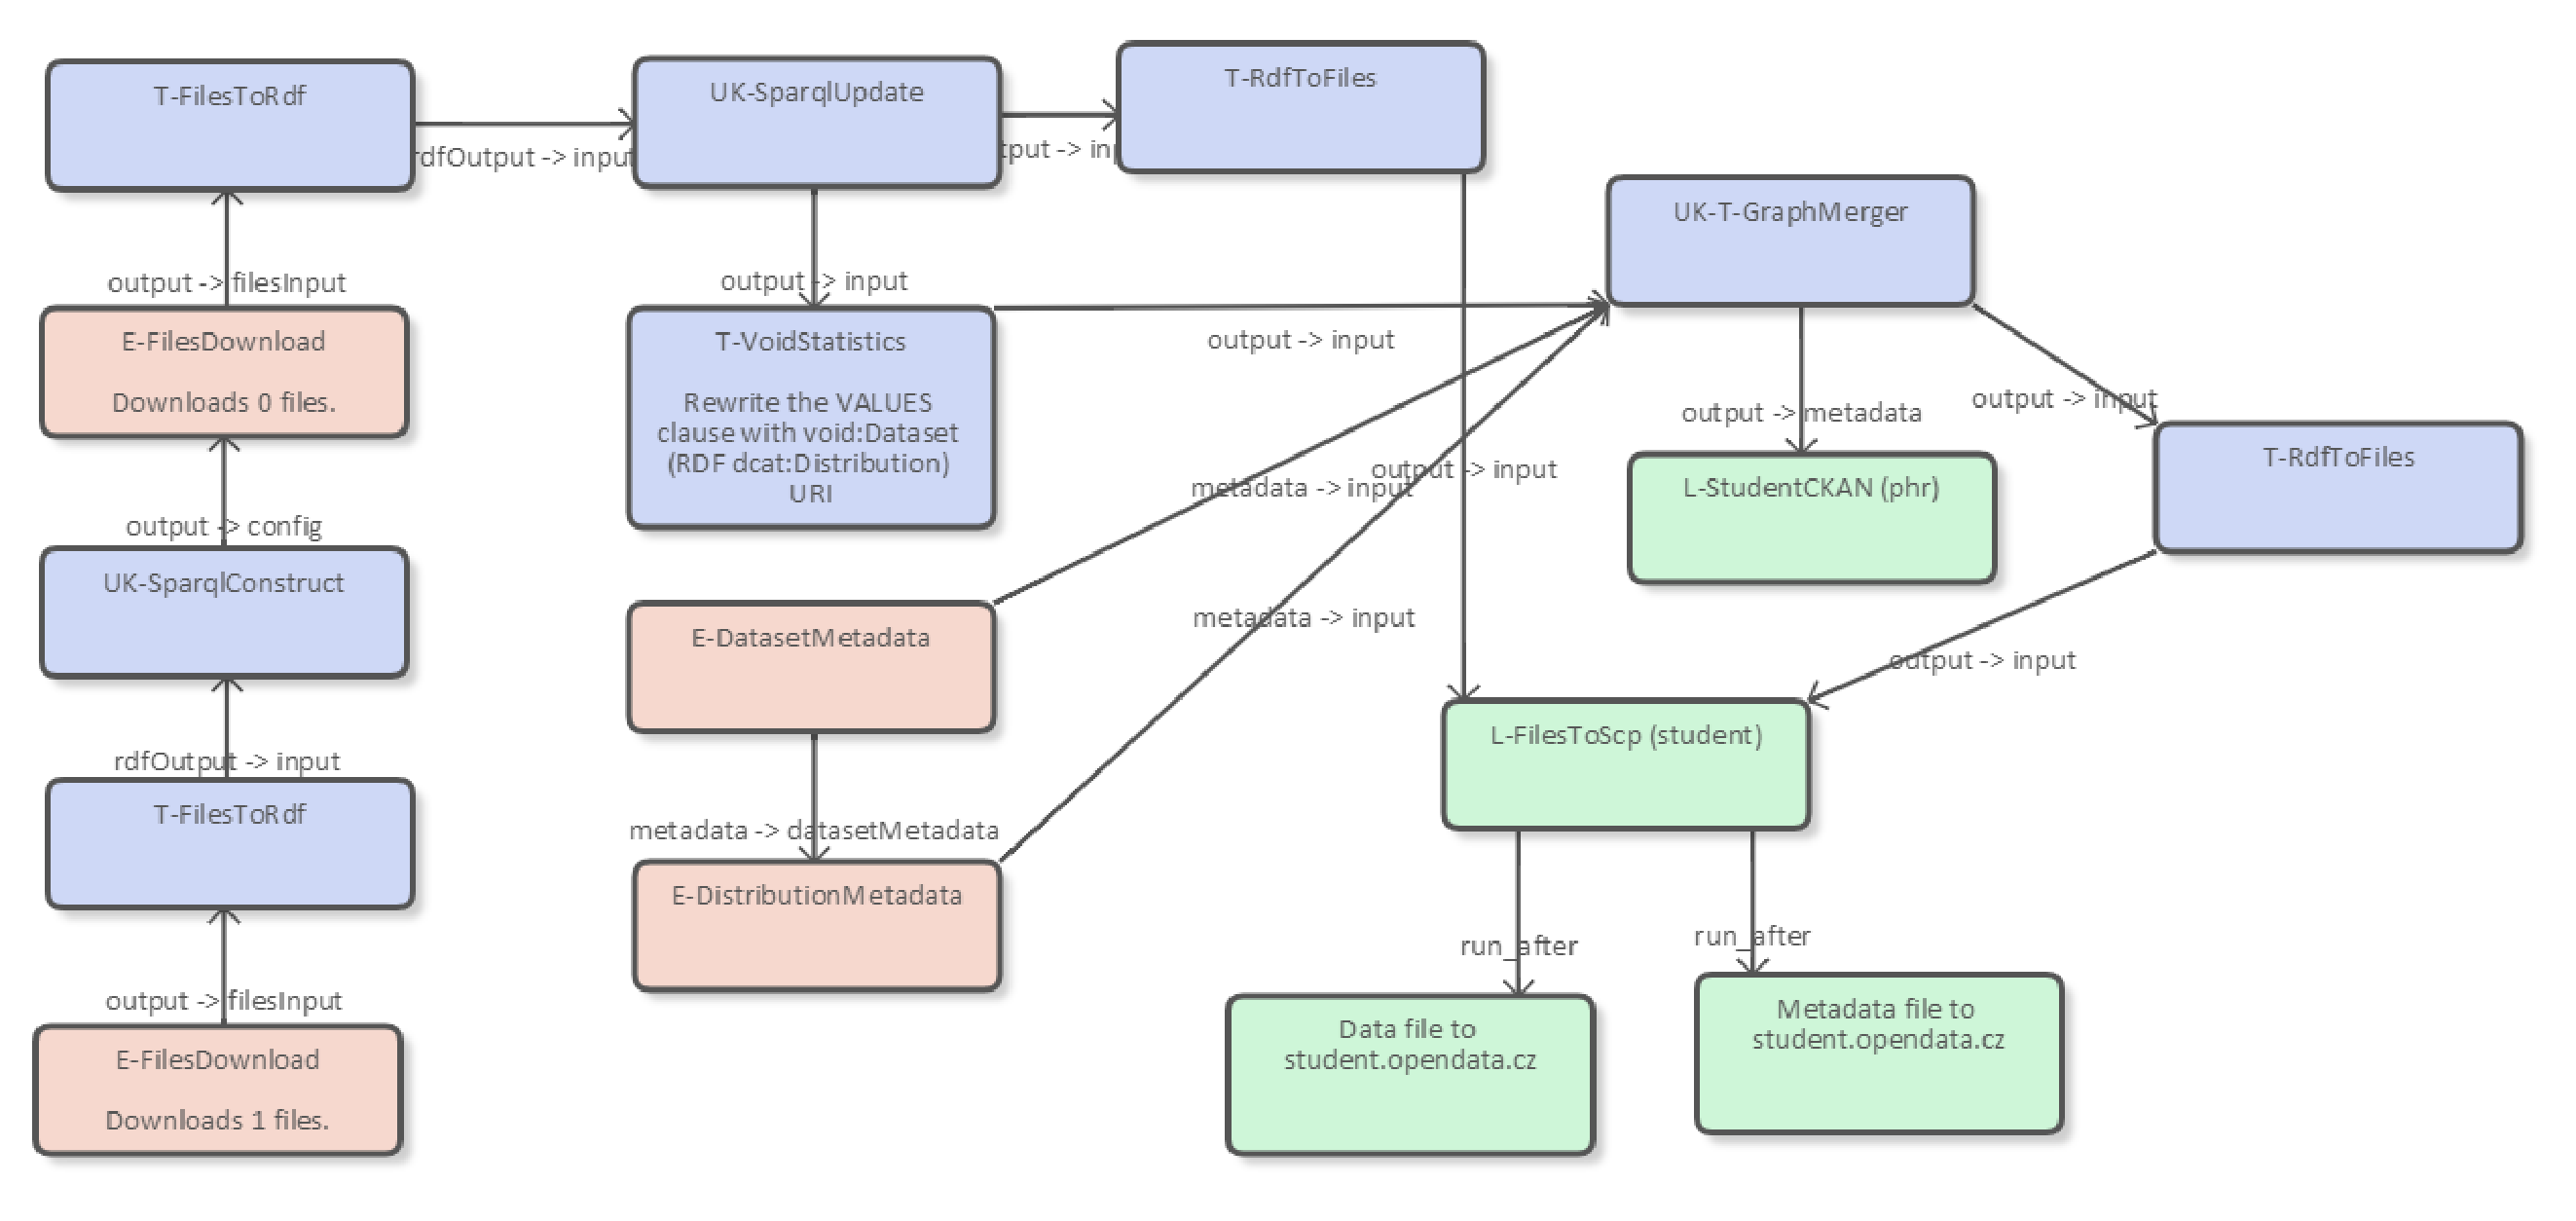
\includegraphics[width=\textwidth]{img/unv.eps}}
\caption{Pipeline nad jednotným úložištěm pro zpracování dat o smlouvách}
\label{obr:unv}
\end{figure}

\subsubsection*{Načtení datového katalogu}

K načtení, resp. zpracování datového katalogu s datasety subjektů slouží první tři DPU pipeliny (viz Obr. \ref{obr:unv} vlevo dole). V rámci prvního DPU - E-FilesDonwload načteme požadovaný datový katalog \ref{lst:subject_catalog}. V druhém DPU - T-FilesToRdf převedeme načtená data do RDF reprezentace. Pokud však chceme pomocí nástroje Unified views dávkově stahovat data, je nutné, aby splňovaly strukturu znázorněnou příkladem kódu \ref{lst:unvConfigurationSample}. Vytvoříme tedy SPARQL příkaz mapující informace z původního datového katalogu do požadované reprezentace (viz Kód \ref{lst:unvLoadCatalog}). Pro tuto funkcionalitu využijeme DPU - UK-SparqlContruct.

\lstinputlisting[label=lst:unvConfigurationSample, caption=Příklad formátu dat pro dávkové zpracování nástrojem UV, language=XML]{code/unvConfigurationSample.ttl}

\lstinputlisting[label=lst:unvLoadCatalog, caption=Příkaz mapující datový katalog do reprezentace nástroje UV, language=XML]{code/unvLoadCatalog.sparql}

\subsubsection*{Zpracování jednotlivých datasetů}

Nyní pomocí DPU - E-FilesDonwload již můžeme stáhnout požadované datasety a pomocí DPU - T-FilesToRdf je převést do RDF reprezentace. V rámci předzpracování provedeme nad daty tuto operaci (v rámci DPU - UK-SparqlUpdate):

\begin{itemize}
\item Obecně subjekt publikující smlouvy nutně nemusí mít podrobné informace o smluvních stranách, ale např. má jen IČ. Za předpokladu, že u smluvních stran je vyplněno jen IČ, tak vytvoříme propojení na odpovídající objekt v Linked Data reprezentaci ekonomického subjektu (Viz Kód\ref{lst:unvPreprocesing}).  
\end{itemize}

\lstinputlisting[label=lst:unvPreprocesing, caption=Příkaz mapující IČ na reprezentaci ekonomického subjektu, language=XML]{code/unvPreprocesing.sparql}

\subsubsection*{Uložení a publikace výsledné datové sady}

V první fázi definujeme Metadata o celé datové sadě reprezentující smlouvy. Popíšeme, k čemu datová sada slouží, jaké má URI, licence apod. K tomu slouží DPU - E-DatasetMetadata a DPU - E-DistributionMetadata. Nad datasetem provedeme také statistické výpočty (počty trojic, entit, tříd atd.) pomocí SPARQL příkazu \ref{lst:unStats} v rámci DPU - T-VoidStatistics. 

\lstinputlisting[label=lst:unStats, caption=Statistické výpočty nad Otevřenými smlouvami, language=XML]{code/unStats.sparql}

V druhé fázi výsledky z těchto DPU slijeme dohromady pomocí DPU - UK-T-GraphMerger. Tímto nám vzniknou úplná metadata o datové sadě otevřených smluv. Tyto informace již můžeme zveřejnit v rejstříku datových sad. V našem případě nad platformou CKAN\cite{ckan} (pomocí DPU - L-StudentCKAN). Datová sada je dostupná na adrese:

\begin{itemize}
\item \textit{http://student.opendata.cz/dataset/phr-contracts }\cite{contractCkan}
\end{itemize}

V poslední, třetí fázi data i metadata serializujeme do výstupních souborů v RDF formátu (obě DPU - T-RdfToFiles) a publikujeme do triplestore databáze Virtuoso Universal Server\cite{virtuoso} (Zbylé DPUs). Vystavený sparql endpoint je dostupný na adrese

\begin{itemize}
\item \textit{http://student.opendata.cz/sparql}
\end{itemize}

\subsection{Požadavky na architekturu}

Databázovým, převodním i publikačním modulem je v našem případě nástroj Unified views. Konfigurací rozumíme jednak nastavení jednotlivých DPU v rámci pipeline, tak načítaný soubor s katalogem požadovaných datových sad. Posledním požadavkem je možnost nastavení intervalu exekuce definované pipeline. V rámci nástroje Unified views k tomu slouží funkce \uv{Schedule a pipeline} (viz Obr. \ref{obr:unvSchedule}).

\begin{figure}[H]
\centerline{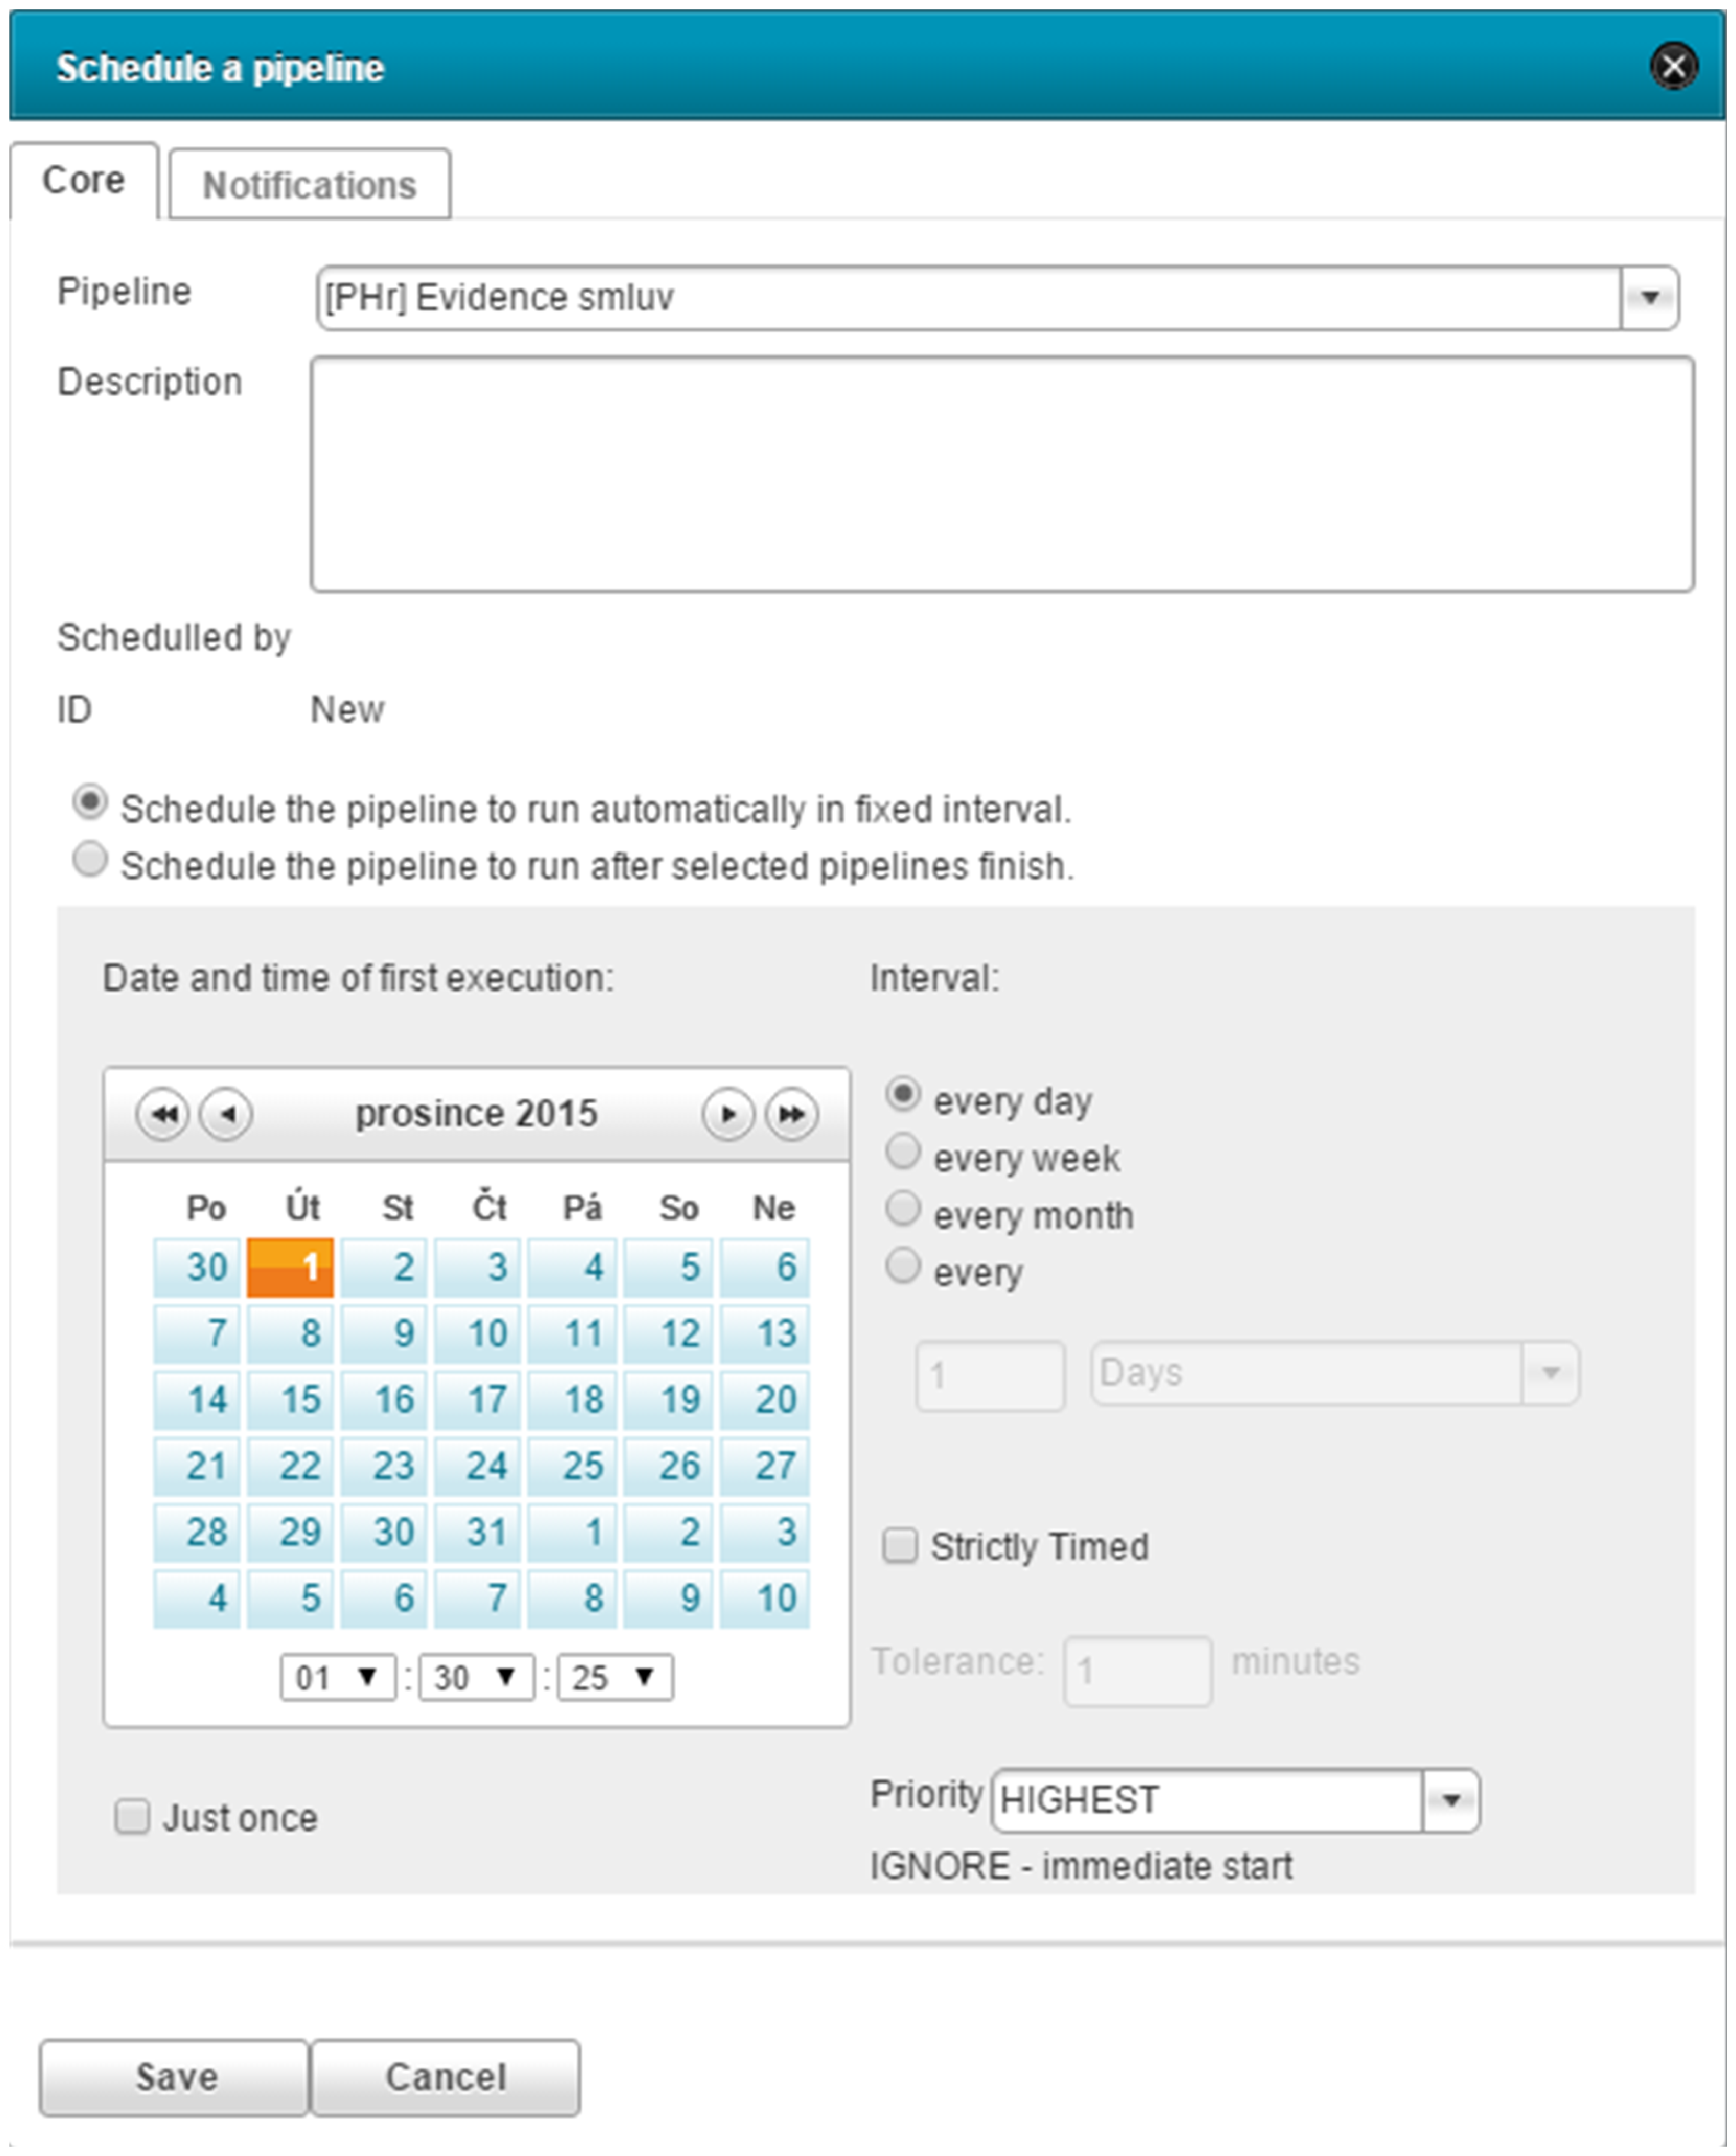
\includegraphics[width=80mm]{img/unvSchedule.eps}}
\caption{Nastavení intervalu exekuze pipeline nástroji UV}
\label{obr:unvSchedule}
\end{figure}

\section{Webová aplikace}

\subsection{Volba technologií a implementační platformy}

Webová aplikace je implementována také v technologii ASP.Net se zvoleným architektonickým vzorem MVC. K práci s RDF daty využijeme také knihovnu dotnetRdf. Layout aplikace je tvořen formou responzivního Bootstrap designu. Aplikace se skládá z pěti pohledů: Úvodní obrazovka, Detail subjektu, Detail smlouvy, Veřejné zakázky subjektu a O aplikaci.

\subsection{Získávání dat}

V rámci aplikace využíváme přístup k datovým sadám z těchto SPARQL endpointů:

\begin{itemize}
\item Otevřené smlouvy - http://student.opendata.cz/sparql
\item Organizace, ARES, Orgány veřejné moci - http://linked.opendata.cz/sparql
\item RÚIAN - http://ruian.linked.opendata.cz/sparql
\item DBpedia - http://dbpedia.org/sparql, nebo česká verze http://cs.dbpedia.org/sparql
\end{itemize}

Konkrétní data se získávají pomocí SPARQL dotazů popsaných níže v rámci popisu jednotlivých pohledů\footnote{Položky uvedené znakem "@" jsou proměnné}.

\subsubsection*{Úvodní obrazovka}

Úvodní obrazovku můžeme rozdělit do pomyslných tří částí. 

První částí je hlavička obsahující odkazy na web Iniciativy za otevřenou datovou infrastrukturu\cite{od}, datový standard pro otevřené smlouvy\cite{metodika} a informace o aplikaci.

Druhou částí je zobrazení vydavatelů na mapovém podkladu. Nejdříve získáme informace o subjektech pomocí SPARQL dotazu \ref{lst:getPublishers} (endpoint Otevřené smlouvy). Posléze pro každý subjekt nalezneme jeho link pro přístup k RÚIANU dotazem \ref{lst:getBusinessEntityRuianLink} (endpoint Organizace, ARES, Orgány veřejné moci). Pomocí obdrženého linku získáme informace o adresním místu z RÚIANu dotazem \ref{lst:getBusinessEntityCoordinates} (endpoint RÚIAN). Na závěr zkusíme získat foto subjektu z DBpedie dotazem \ref{lst:getPublisherImage} (endpoint DBpedia). Získané informace zobrazíme uživateli na mapovém podkladu. Každý subjekt je zvýrazněn na svých souřadnicích\footnote{Počet otevřených smluv je v mapě znázorněn červeným kruhem. Ti, co jich mají více, jsou výraznější.}. Po kliku na subjekt se otevře informační okno s podrobnostmi s možností přejití na detail subjektu.

Třetí částí je seznam smluv. Smlouvy získáme pomocí SPARQL dotazu \ref{lst:getContracts} (endpoint Otevřené smlouvy) (Viz Obr. \ref{obr:mainPage}).\\

\begin{figure}[H]
\centerline{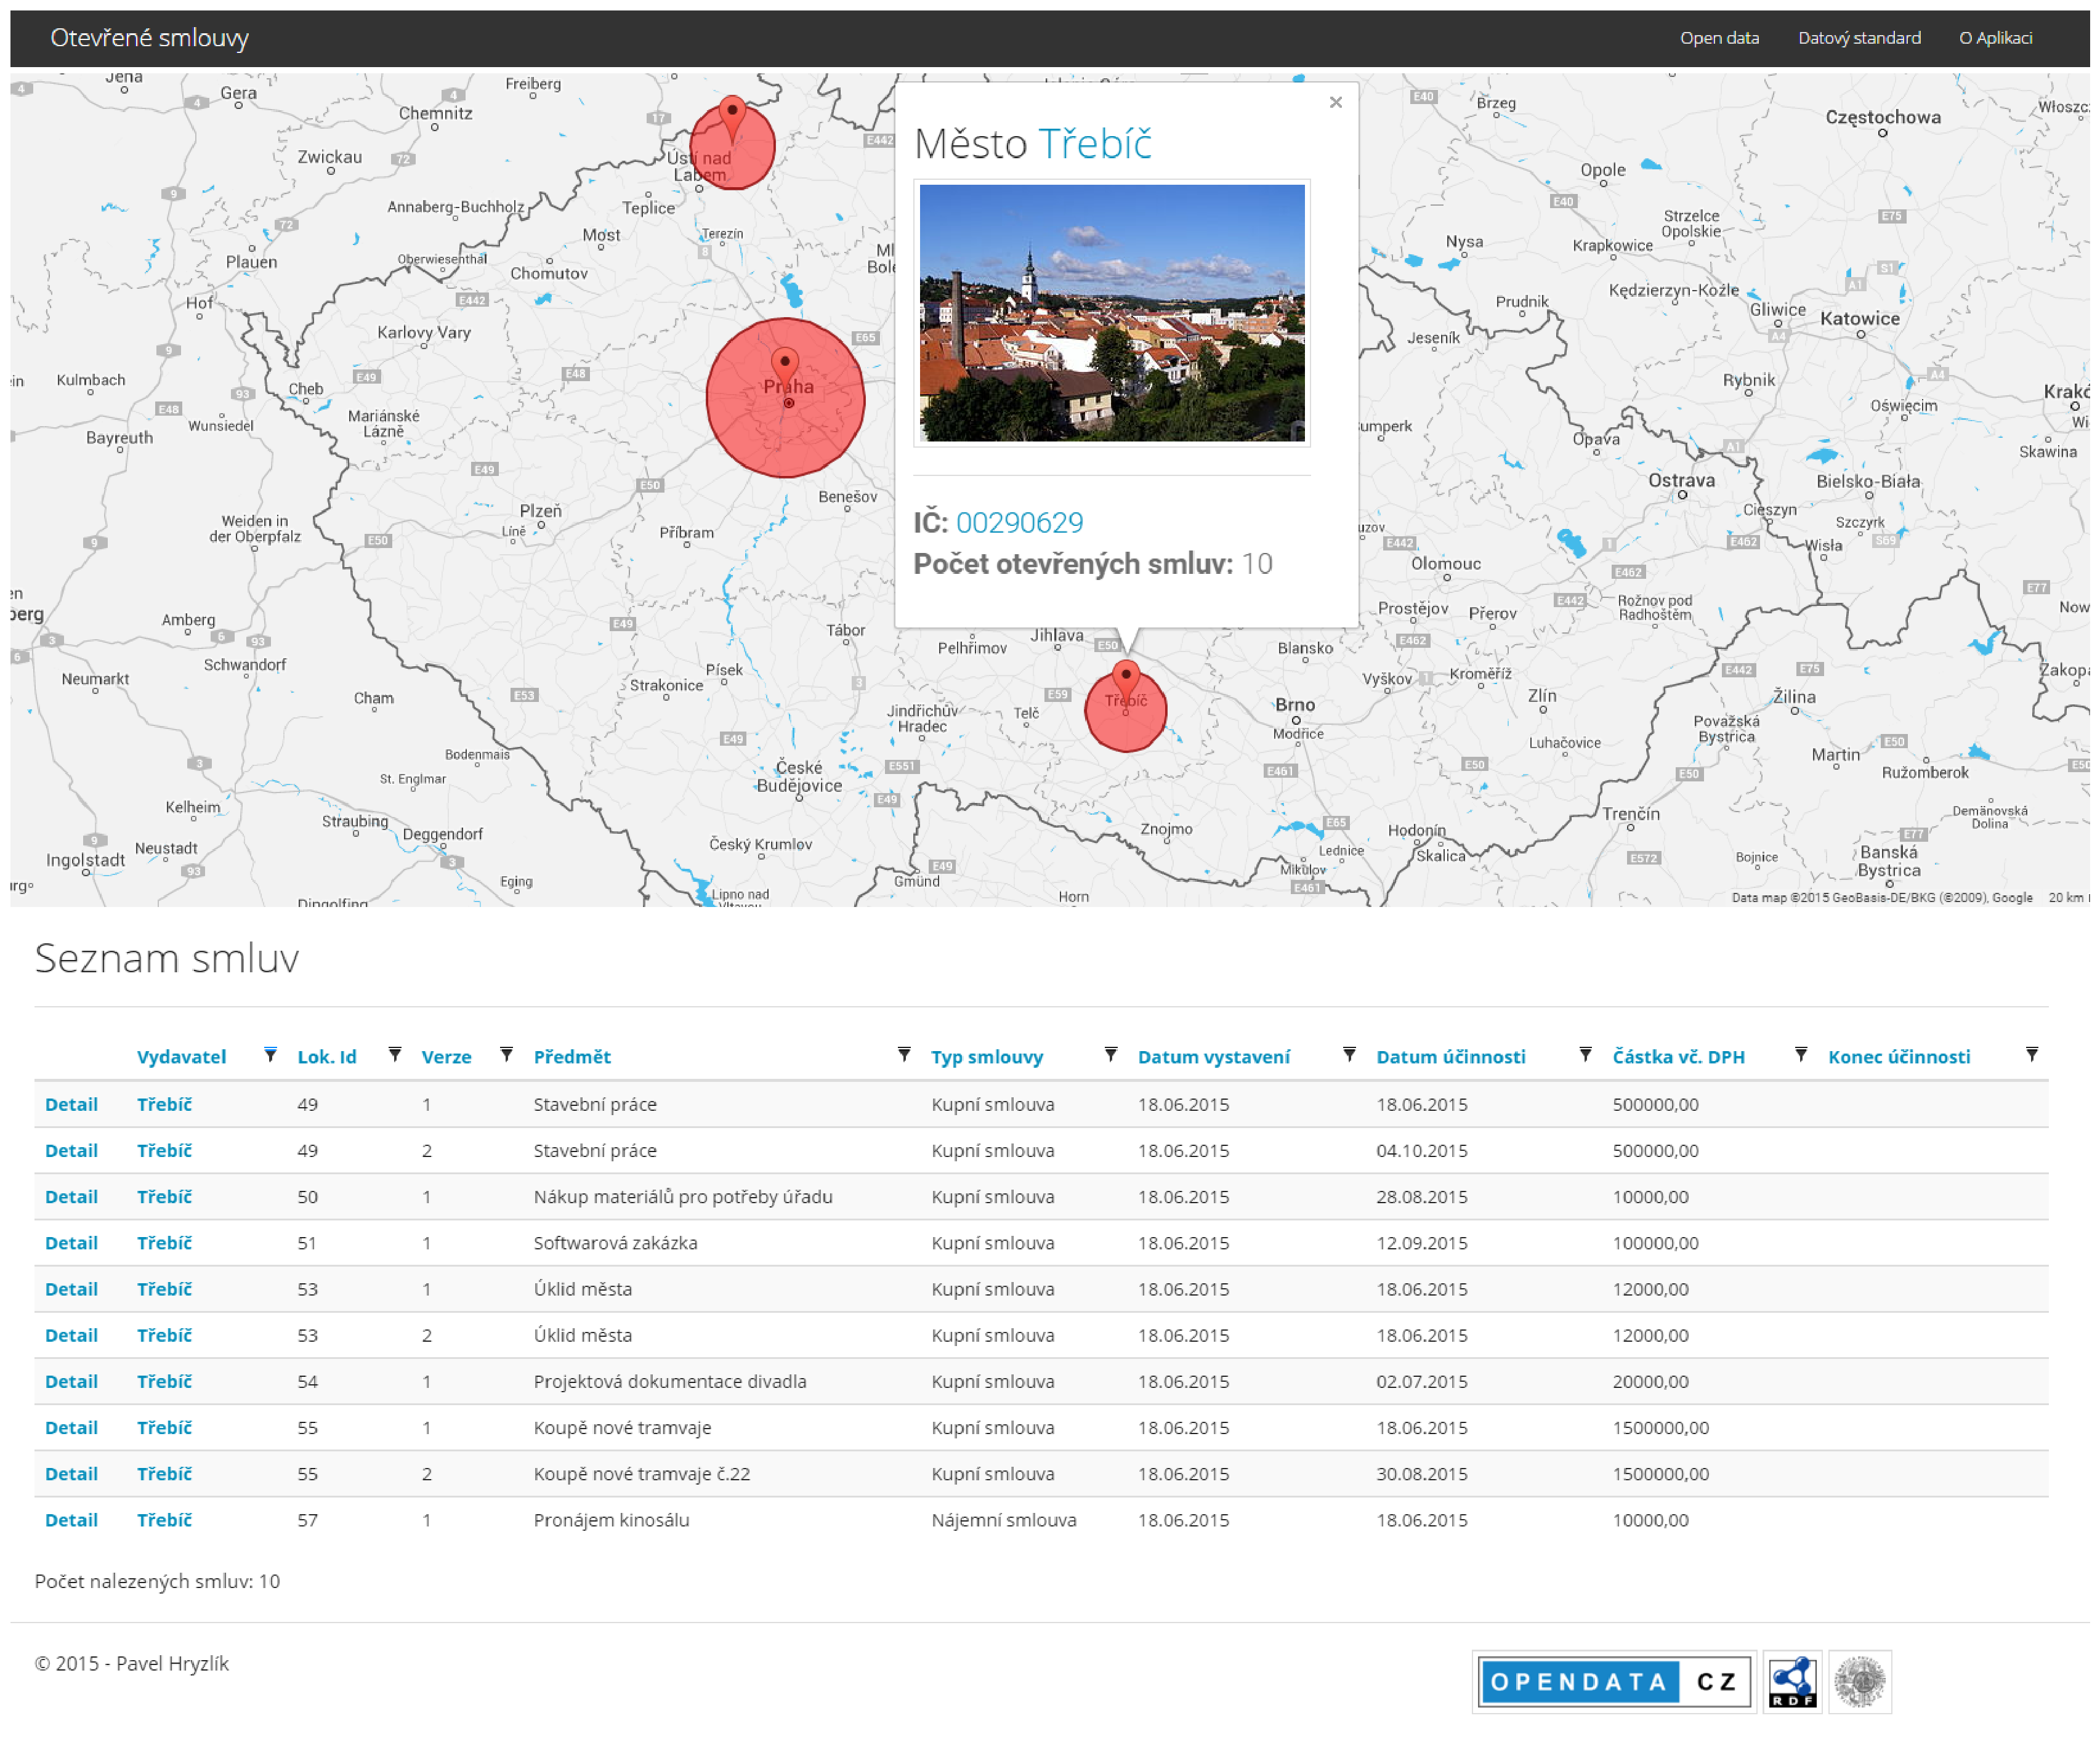
\includegraphics[width=\textwidth]{img/webMainPage.eps}}
\caption{Úvodní obrazovka webové aplikace}
\label{obr:mainPage}
\end{figure}

\lstinputlisting[label=lst:getPublishers, caption=Získej informace o subjektech, language=XML]{code/getPublishers.sparql}

\lstinputlisting[label=lst:getBusinessEntityRuianLink, caption=Získej adresní místo, language=XML]{code/getBusinessEntityRuianLink.sparql}

\lstinputlisting[label=lst:getBusinessEntityCoordinates, caption=Získej polohu subjektu, language=XML]{code/getBusinessEntityCoordinates.sparql}

\lstinputlisting[label=lst:getPublisherImage, caption=Získej foto subjektu, language=XML]{code/getPublisherImage.sparql}

\lstinputlisting[label=lst:getContracts, caption=Získej všechny smlouvy, language=XML]{code/getContracts.sparql}

\subsubsection*{Detail subjektu}

Detail subjektu nabízí podrobné informace o vydavateli a seznam jeho smluv. Informace o subjektu získáme na základě jeho IČ dotazem \ref{lst:getPublisherByIc} (endpoint Otevřené smlouvy). Další informace získáme podobně jako na úvodní obrazovce dotazy \ref{lst:getBusinessEntityRuianLink},\ref{lst:getPublisherImage}. Jako informaci navíc zkusíme zjistit informace o otevíracích dobách vydavatele dotazem \ref{lst:getBusinessEntityOpeningHours} (endpoint Organizace, ARES, Orgány veřejné moci). Posléze nad endpointem Otevřené smlouvy obdržíme seznam smluv subjektu pomocí dotazu \ref{lst:getContractByPublisheIc} (Viz Obr. \ref{obr:webSubjectDetail}).\\

\begin{figure}[H]
\centerline{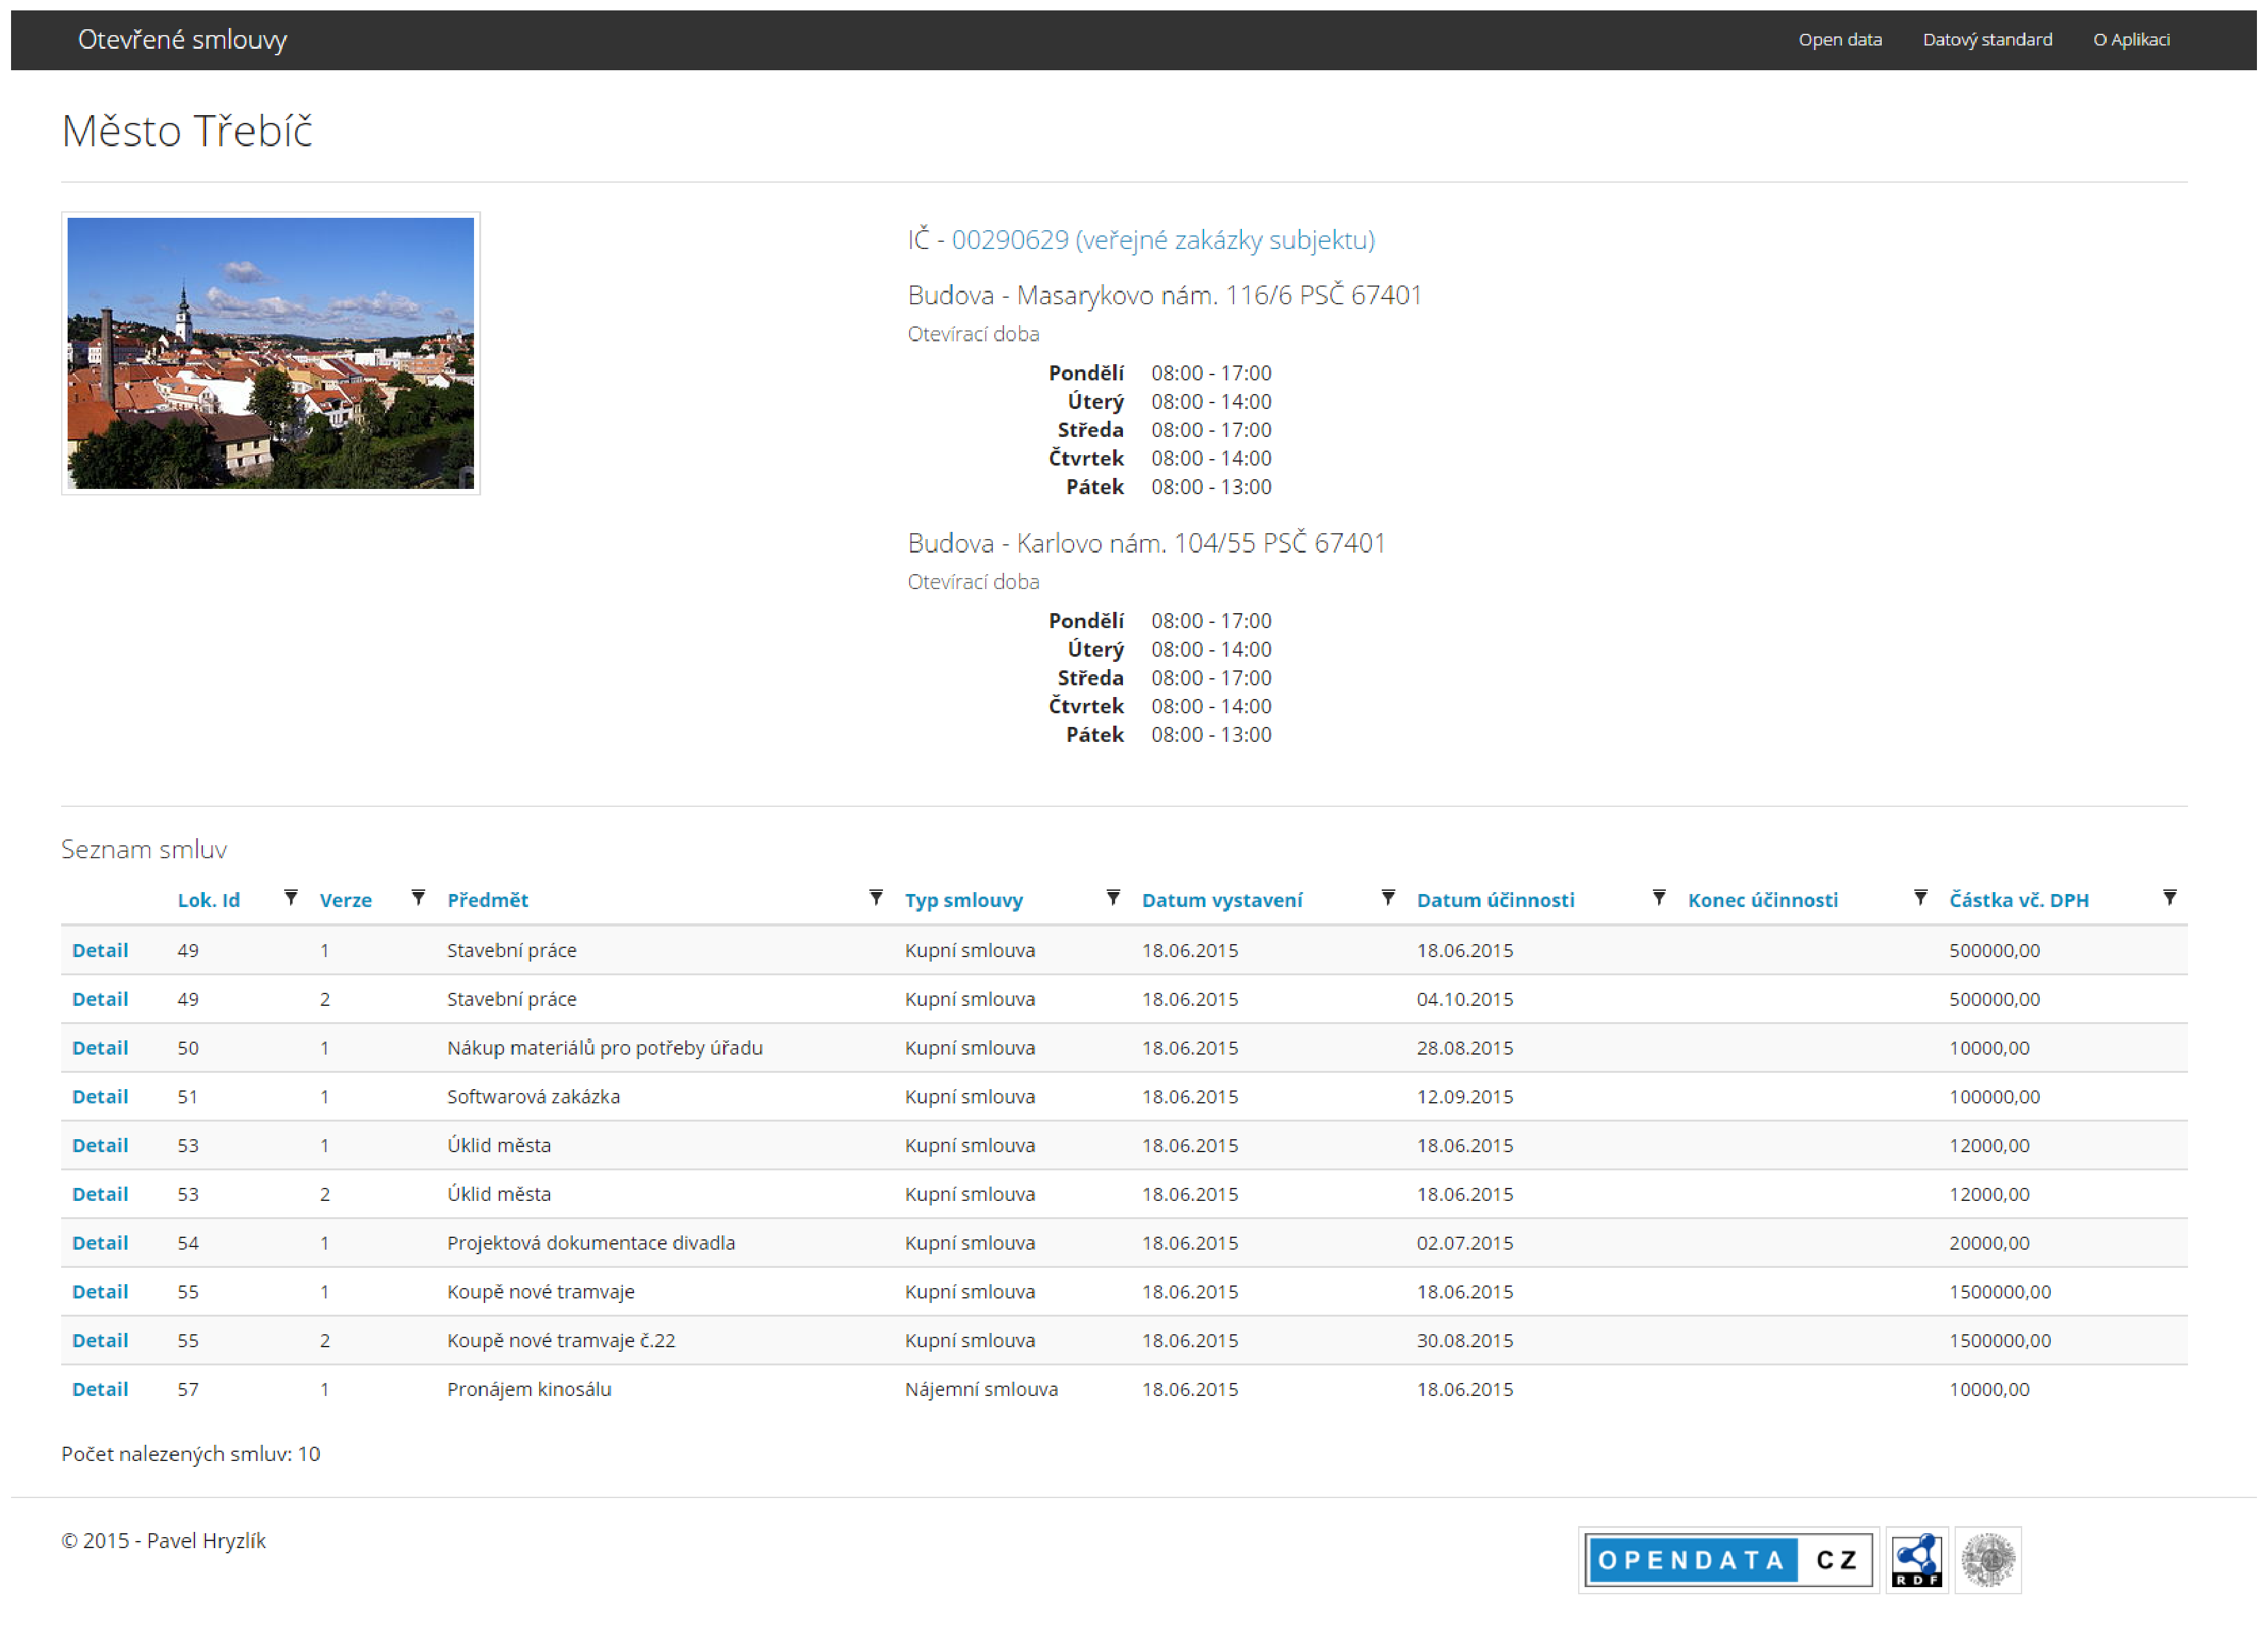
\includegraphics[width=\textwidth]{img/webSubjectDetail.eps}}
\caption{Obrazovka detailu subjektu}
\label{obr:webSubjectDetail}
\end{figure}

\lstinputlisting[label=lst:getPublisherByIc, caption=Získej vydavatele na základě IČ, language=XML]{code/getPublisherByIc.sparql}

\lstinputlisting[label=lst:getBusinessEntityOpeningHours, caption=Získej otevírací hodiny subjektu, language=XML]{code/getBusinessEntityOpeningHours.sparql}

\lstinputlisting[label=lst:getContractByPublisheIc, caption=Získej všechny smlouvy daného vydavatele, language=XML]{code/getContractByPublisheIc.sparql}


\subsubsection*{Detail smlouvy}

Jak název napovídá, detail smlouvy poskytuje podrobné informace o smlouvě, smluvních stranách, přílohách, dodatcích, milnících, informacích o ceně a verzích smlouvy. Údaje získáme pomocí dotazů \ref{lst:getContract},\ref{lst:getPartiesByContract},\ref{lst:getAttachmentsByContract},\ref{lst:getAmendmentsByContract},\ref{lst:getMilestonesByContract},\ref{lst:getPriceSpecByContract},\ref{lst:getVersionsByContract} nad endpointem Otevřené smlouvy (Viz Obr. \ref{obr:contractDetail}).\\

\begin{figure}[H]
\centerline{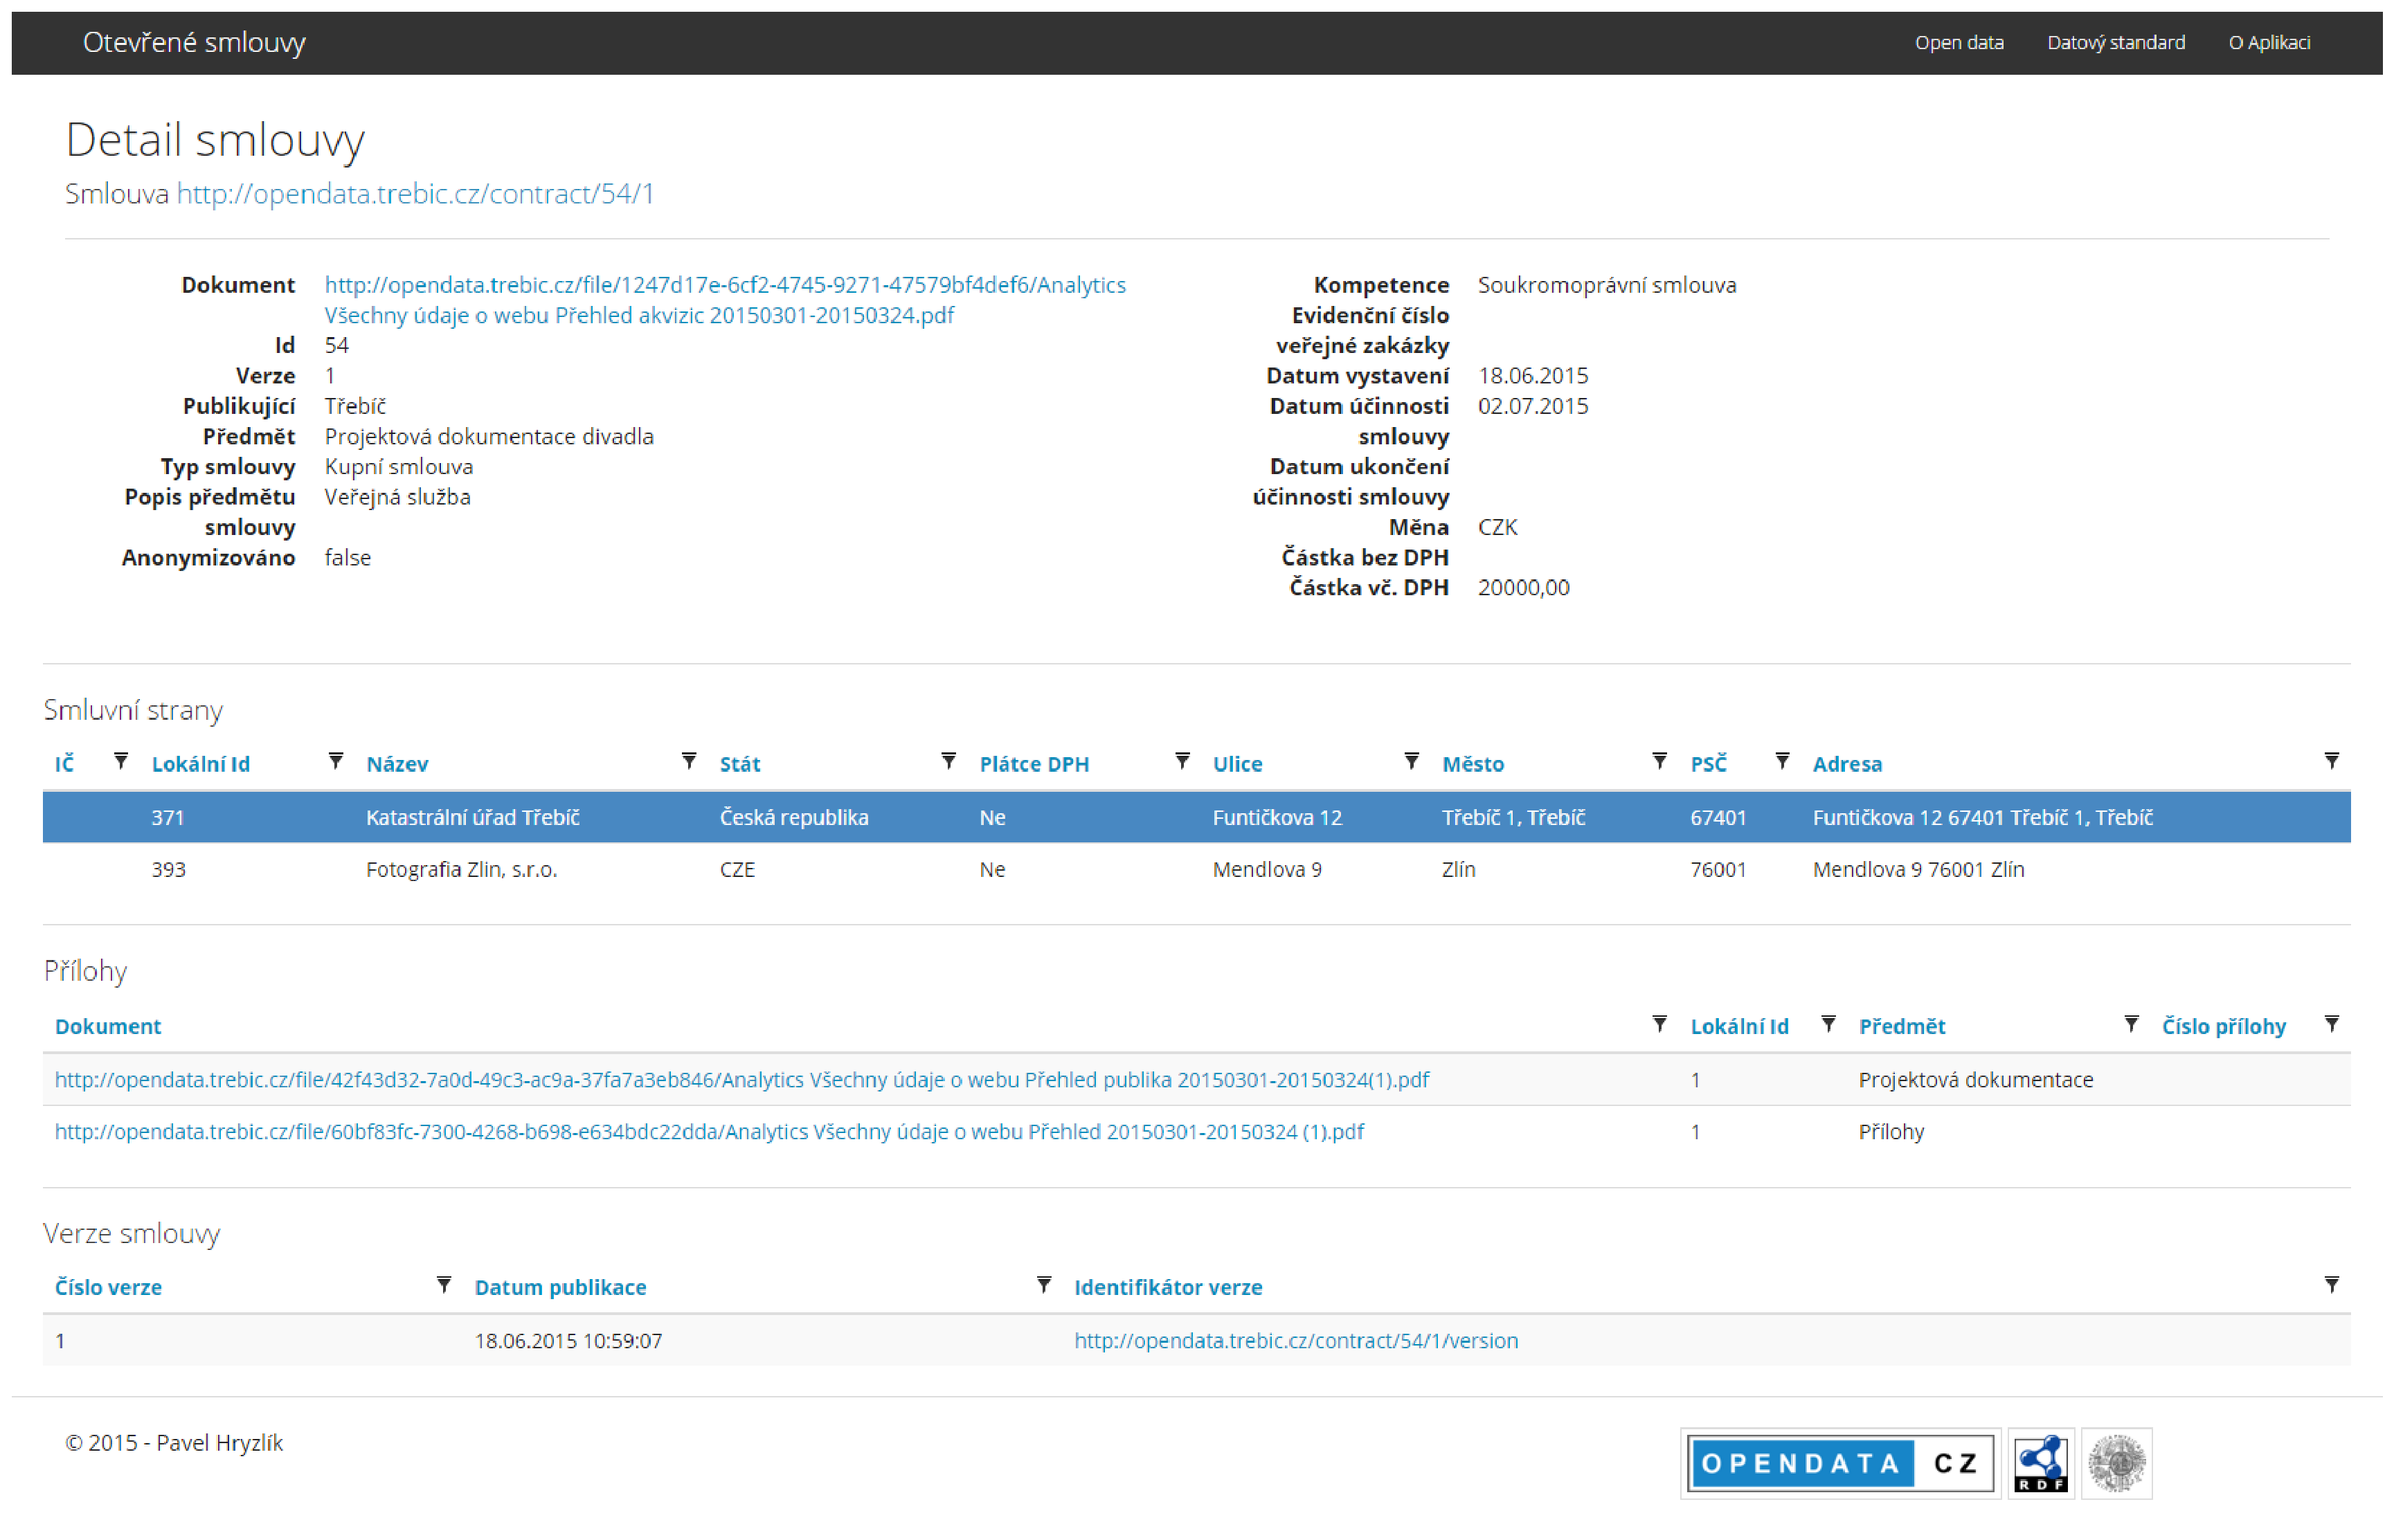
\includegraphics[width=\textwidth]{img/webContractDetail.eps}}
\caption{Obrazovka detailu smlouvy}
\label{obr:contractDetail}
\end{figure}

\lstinputlisting[label=lst:getContract, caption=Získej smlouvu, language=XML]{code/getContract.sparql}

\lstinputlisting[label=lst:getPartiesByContract, caption=Získej smluvní strany na základě smlouvy, language=XML]{code/getPartiesByContract.sparql}

\lstinputlisting[label=lst:getAttachmentsByContract, caption=Získej přílohy na základě smlouvy, language=XML]{code/getAttachmentsByContract.sparql}

\lstinputlisting[label=lst:getAmendmentsByContract, caption=Získej dodatky na základě smlouvy, language=XML]{code/getAmendmentsByContract.sparql}

\lstinputlisting[label=lst:getMilestonesByContract, caption=Získej milníky na základě smlouvy, language=XML]{code/getMilestonesByContract.sparql}

\lstinputlisting[label=lst:getPriceSpecByContract, caption=Získej informace o ceně, language=XML]{code/getPriceSpecByContract.sparql}

\lstinputlisting[label=lst:getVersionsByContract, caption=Získej verze smlouvy, language=XML]{code/getVersionsByContract.sparql}


\subsubsection*{Veřejné zakázky subjektu}

Seznam veřejných zakázek je dostupný z detailu subjektu na základě jeho IČ. Získáme jej dotazem \ref{lst:getBusinessEntityPublicContracts} (endpoint Organizace, ARES, Orgány veřejné moci) (Viz Obr. \ref{obr:webPublicContracts}).\\

\begin{figure}[H]
\centerline{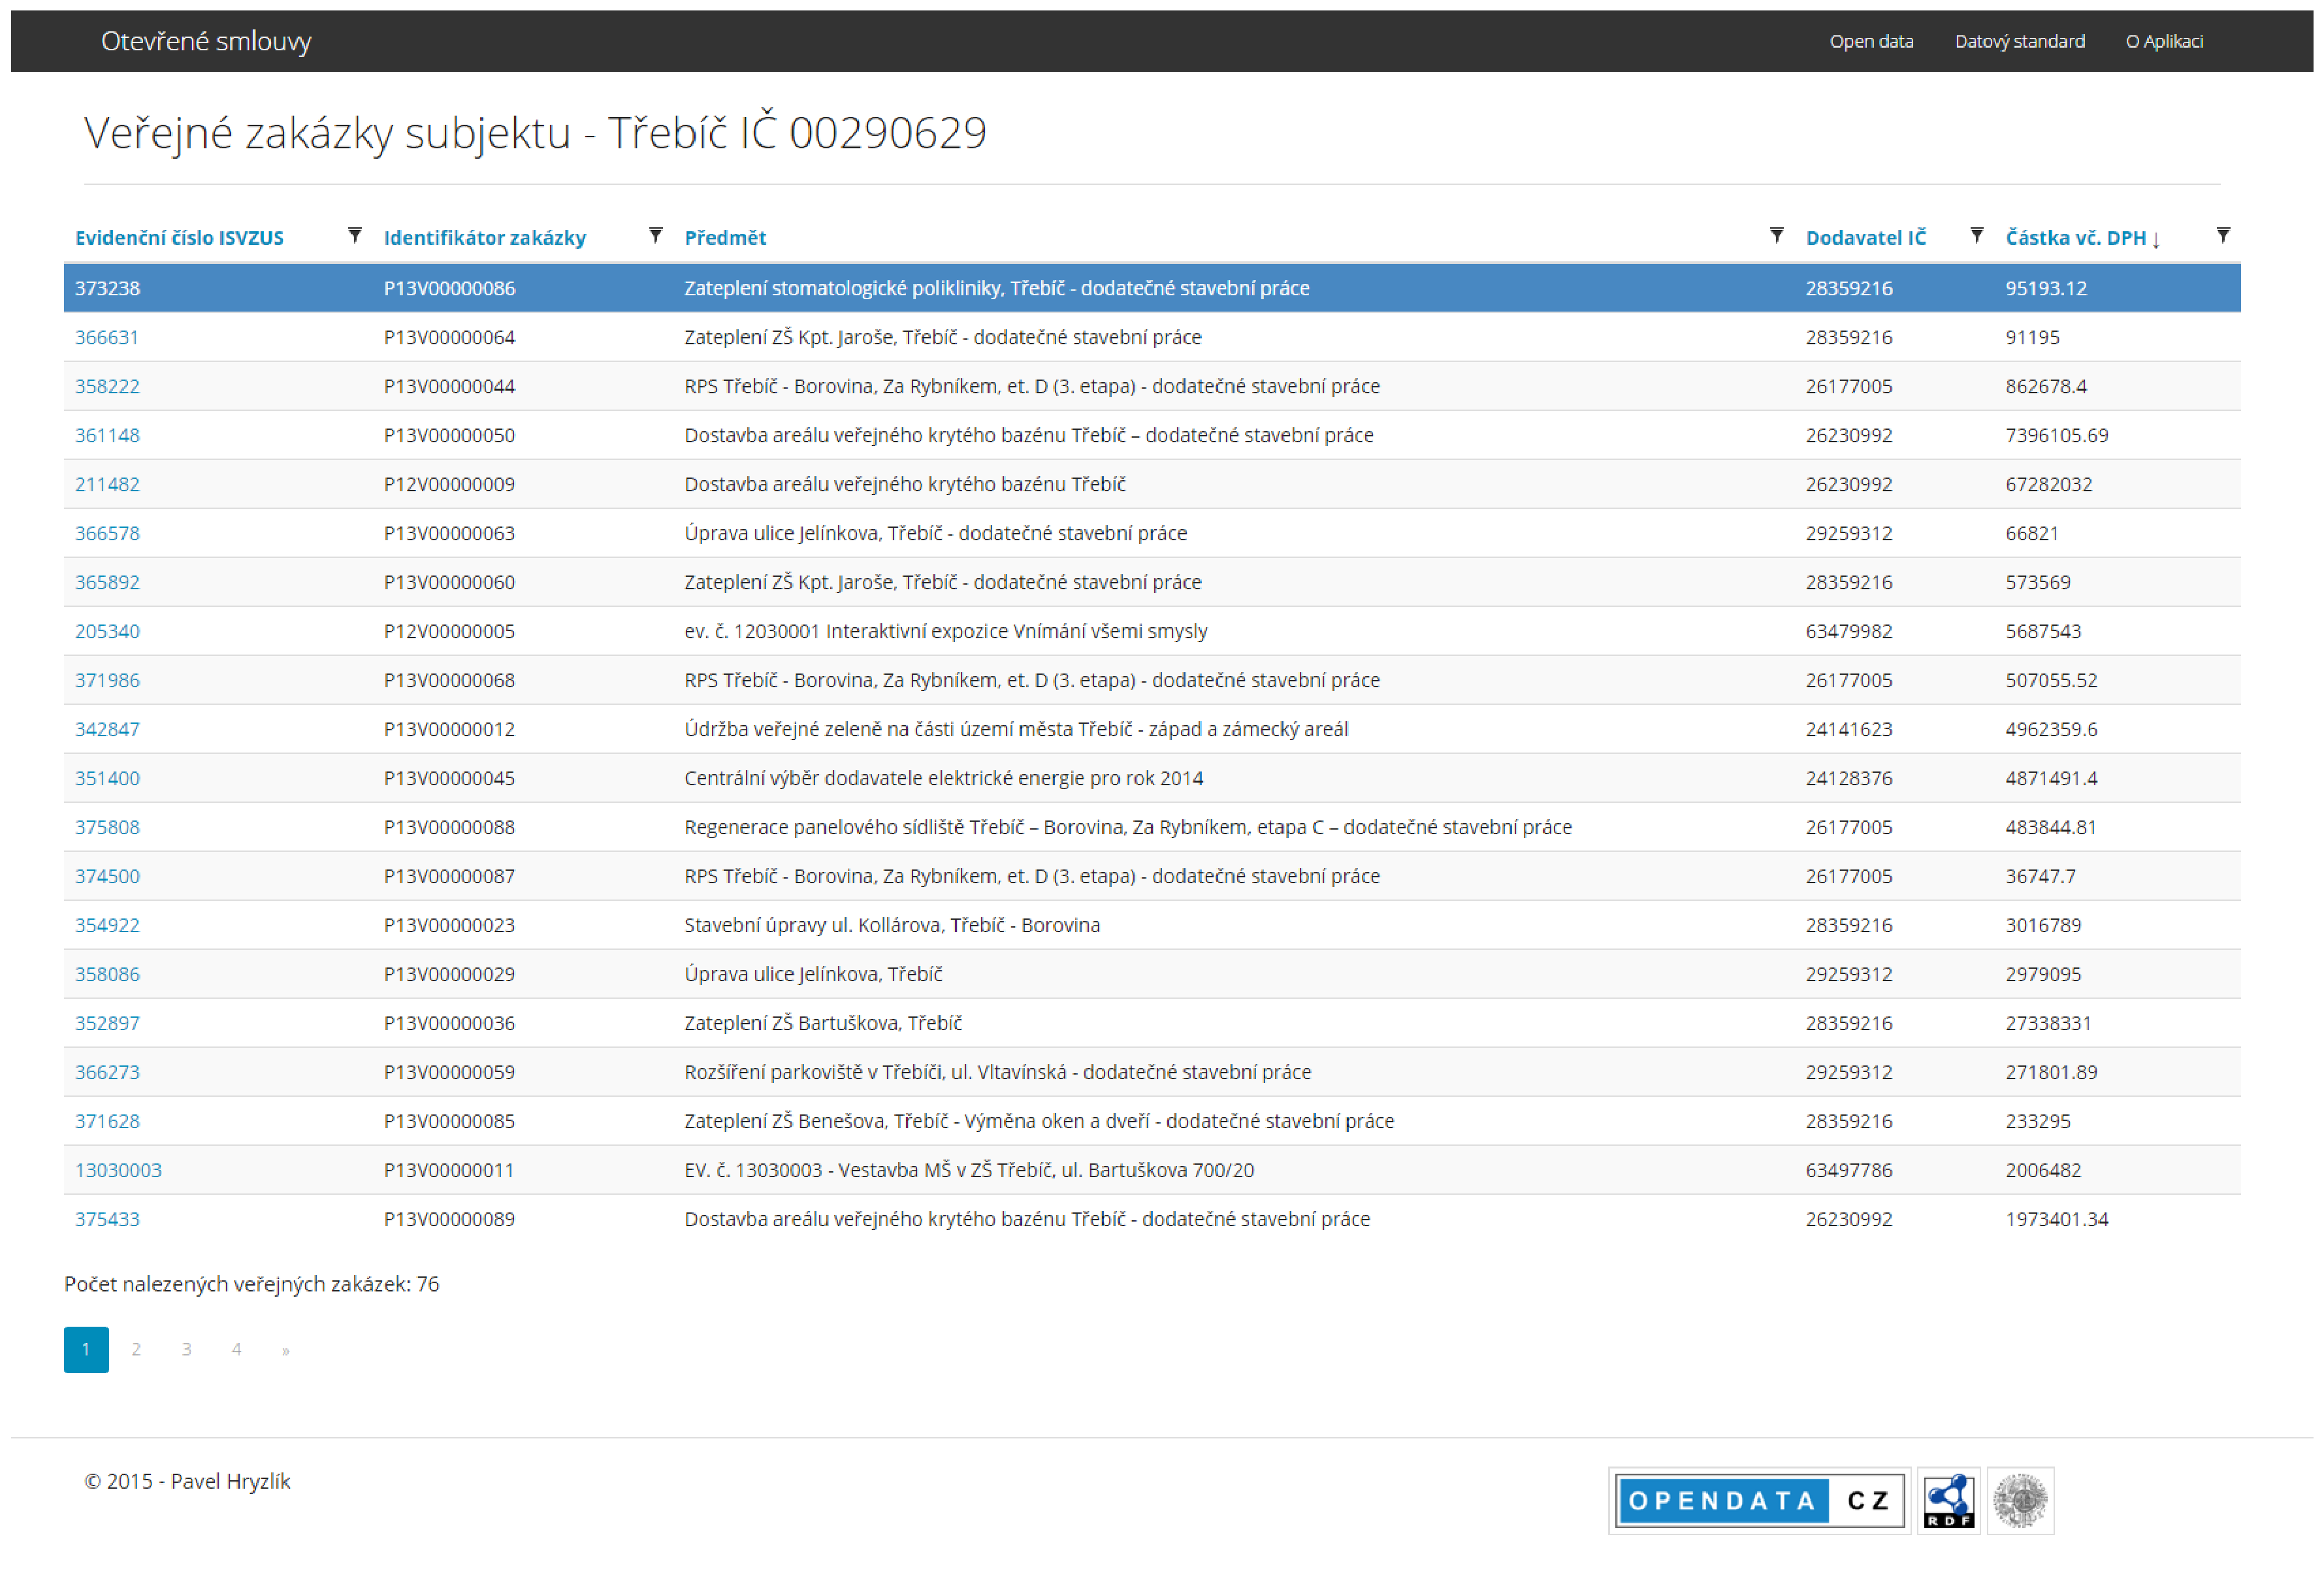
\includegraphics[width=\textwidth]{img/webPublicContracts.eps}}
\caption{Obrazovka seznamu veřejných zakázek subjektu}
\label{obr:webPublicContracts}
\end{figure}

\lstinputlisting[label=lst:getBusinessEntityPublicContracts, caption=Získej veřejné zakázky na základě subjektu, language=XML]{code/getBusinessEntityPublicContracts.sparql}

\subsubsection*{O aplikaci}

V rámci tohoto pohledu jsou uvedeny základní informace o projektu.

\subsection{Požadavky na architekturu}

Pro implementaci jsme zvolili technologii ASP.Net s architektonickým vzorem MVC. Procesním a endpoint modulem je tedy v tomto případě Controller, který na základě klientských požadavků volá odpovídající SPARQL dotazy získávající data z různých zdrojů (endpointů). Komunikace mezi procesním a prezentačním modelem (Komunikační modul) je řešena interně v rámci technologie ASP.Net. V rámci architektury MVC je prezentačním modulem část View obsahující jednotlivé pohledy popsané výše.


